
%% bare_jrnl.tex
%% V1.4a
%% 2014/09/17
%% by Michael Shell
%% see http://www.michaelshell.org/
%% for current contact information.
%%
%% This is a skeleton file demonstrating the use of IEEEtran.cls
%% (requires IEEEtran.cls version 1.8a or later) with an IEEE
%% journal paper.
%%
%% Support sites:
%% http://www.michaelshell.org/tex/ieeetran/
%% http://www.ctan.org/tex-archive/macros/latex/contrib/IEEEtran/
%% and
%% http://www.ieee.org/

%%*************************************************************************
%% Legal Notice:
%% This code is offered as-is without any warranty either expressed or
%% implied; without even the implied warranty of MERCHANTABILITY or
%% FITNESS FOR A PARTICULAR PURPOSE! 
%% User assumes all risk.
%% In no event shall IEEE or any contributor to this code be liable for
%% any damages or losses, including, but not limited to, incidental,
%% consequential, or any other damages, resulting from the use or misuse
%% of any information contained here.
%%
%% All comments are the opinions of their respective authors and are not
%% necessarily endorsed by the IEEE.
%%
%% This work is distributed under the LaTeX Project Public License (LPPL)
%% ( http://www.latex-project.org/ ) version 1.3, and may be freely used,
%% distributed and modified. A copy of the LPPL, version 1.3, is included
%% in the base LaTeX documentation of all distributions of LaTeX released
%% 2003/12/01 or later.
%% Retain all contribution notices and credits.
%% ** Modified files should be clearly indicated as such, including  **
%% ** renaming them and changing author support contact information. **
%%
%% File list of work: IEEEtran.cls, IEEEtran_HOWTO.pdf, bare_adv.tex,
%%                    bare_conf.tex, bare_jrnl.tex, bare_conf_compsoc.tex,
%%                    bare_jrnl_compsoc.tex, bare_jrnl_transmag.tex
%%*************************************************************************


% *** Authors should verify (and, if needed, correct) their LaTeX system  ***
% *** with the testflow diagnostic prior to trusting their LaTeX platform ***
% *** with production work. IEEE's font choices and paper sizes can       ***
% *** trigger bugs that do not appear when using other class files.       ***                          ***
% The testflow support page is at:
% http://www.michaelshell.org/tex/testflow/



% \documentclass[journal]{IEEEtran}
%
% If IEEEtran.cls has not been installed into the LaTeX system files,
% manually specify the path to it like:
\documentclass[journal]{IEEEtran}


\usepackage{booktabs}


% Some very useful LaTeX packages include:
% (uncomment the ones you want to load)


% *** MISC UTILITY PACKAGES ***
%
%\usepackage{ifpdf}
% Heiko Oberdiek's ifpdf.sty is very useful if you need conditional
% compilation based on whether the output is pdf or dvi.
% usage:
% \ifpdf
%   % pdf code
% \else
%   % dvi code
% \fi
% The latest version of ifpdf.sty can be obtained from:
% http://www.ctan.org/tex-archive/macros/latex/contrib/oberdiek/
% Also, note that IEEEtran.cls V1.7 and later provides a builtin
% \ifCLASSINFOpdf conditional that works the same way.
% When switching from latex to pdflatex and vice-versa, the compiler may
% have to be run twice to clear warning/error messages.






% *** CITATION PACKAGES ***
%
\usepackage{cite}
% cite.sty was written by Donald Arseneau
% V1.6 and later of IEEEtran pre-defines the format of the cite.sty package
% \cite{} output to follow that of IEEE. Loading the cite package will
% result in citation numbers being automatically sorted and properly
% "compressed/ranged". e.g., [1], [9], [2], [7], [5], [6] without using
% cite.sty will become [1], [2], [5]--[7], [9] using cite.sty. cite.sty's
% \cite will automatically add leading space, if needed. Use cite.sty's
% noadjust option (cite.sty V3.8 and later) if you want to turn this off
% such as if a citation ever needs to be enclosed in parenthesis.
% cite.sty is already installed on most LaTeX systems. Be sure and use
% version 5.0 (2009-03-20) and later if using hyperref.sty.
% The latest version can be obtained at:
% http://www.ctan.org/tex-archive/macros/latex/contrib/cite/
% The documentation is contained in the cite.sty file itself.



\usepackage{csquotes}


% *** GRAPHICS RELATED PACKAGES ***
%
\ifCLASSINFOpdf
  \usepackage[pdftex]{graphicx}
  % declare the path(s) where your graphic files are
  \graphicspath{{/home/chiroptera/workspace/thesis_writing/rsc/}}
  % and their extensions so you won't have to specify these with
  % every instance of \includegraphics
  % \DeclareGraphicsExtensions{.pdf,.jpeg,.png}
\else
  % or other class option (dvipsone, dvipdf, if not using dvips). graphicx
  % will default to the driver specified in the system graphics.cfg if no
  % driver is specified.
  % \usepackage[dvips]{graphicx}
  % declare the path(s) where your graphic files are
  % \graphicspath{{../eps/}}
  % and their extensions so you won't have to specify these with
  % every instance of \includegraphics
  % \DeclareGraphicsExtensions{.eps}
\fi
% graphicx was written by David Carlisle and Sebastian Rahtz. It is
% required if you want graphics, photos, etc. graphicx.sty is already
% installed on most LaTeX systems. The latest version and documentation
% can be obtained at: 
% http://www.ctan.org/tex-archive/macros/latex/required/graphics/
% Another good source of documentation is "Using Imported Graphics in
% LaTeX2e" by Keith Reckdahl which can be found at:
% http://www.ctan.org/tex-archive/info/epslatex/
%
% latex, and pdflatex in dvi mode, support graphics in encapsulated
% postscript (.eps) format. pdflatex in pdf mode supports graphics
% in .pdf, .jpeg, .png and .mps (metapost) formats. Users should ensure
% that all non-photo figures use a vector format (.eps, .pdf, .mps) and
% not a bitmapped formats (.jpeg, .png). IEEE frowns on bitmapped formats
% which can result in "jaggedy"/blurry rendering of lines and letters as
% well as large increases in file sizes.
%
% You can find documentation about the pdfTeX application at:
% http://www.tug.org/applications/pdftex





% *** MATH PACKAGES ***
%
\usepackage[cmex10]{amsmath}
\usepackage{amsfonts}
% A popular package from the American Mathematical Society that provides
% many useful and powerful commands for dealing with mathematics. If using
% it, be sure to load this package with the cmex10 option to ensure that
% only type 1 fonts will utilized at all point sizes. Without this option,
% it is possible that some math symbols, particularly those within
% footnotes, will be rendered in bitmap form which will result in a
% document that can not be IEEE Xplore compliant!
%
% Also, note that the amsmath package sets \interdisplaylinepenalty to 10000
% thus preventing page breaks from occurring within multiline equations. Use:
%\interdisplaylinepenalty=2500
% after loading amsmath to restore such page breaks as IEEEtran.cls normally
% does. amsmath.sty is already installed on most LaTeX systems. The latest
% version and documentation can be obtained at:
% http://www.ctan.org/tex-archive/macros/latex/required/amslatex/math/





% *** SPECIALIZED LIST PACKAGES ***
%
%\usepackage{algorithmic}
% algorithmic.sty was written by Peter Williams and Rogerio Brito.
% This package provides an algorithmic environment fo describing algorithms.
% You can use the algorithmic environment in-text or within a figure
% environment to provide for a floating algorithm. Do NOT use the algorithm
% floating environment provided by algorithm.sty (by the same authors) or
% algorithm2e.sty (by Christophe Fiorio) as IEEE does not use dedicated
% algorithm float types and packages that provide these will not provide
% correct IEEE style captions. The latest version and documentation of
% algorithmic.sty can be obtained at:
% http://www.ctan.org/tex-archive/macros/latex/contrib/algorithms/
% There is also a support site at:
% http://algorithms.berlios.de/index.html
% Also of interest may be the (relatively newer and more customizable)
% algorithmicx.sty package by Szasz Janos:
% http://www.ctan.org/tex-archive/macros/latex/contrib/algorithmicx/




% *** ALIGNMENT PACKAGES ***
%
%\usepackage{array}
% Frank Mittelbach's and David Carlisle's array.sty patches and improves
% the standard LaTeX2e array and tabular environments to provide better
% appearance and additional user controls. As the default LaTeX2e table
% generation code is lacking to the point of almost being broken with
% respect to the quality of the end results, all users are strongly
% advised to use an enhanced (at the very least that provided by array.sty)
% set of table tools. array.sty is already installed on most systems. The
% latest version and documentation can be obtained at:
% http://www.ctan.org/tex-archive/macros/latex/required/tools/


% IEEEtran contains the IEEEeqnarray family of commands that can be used to
% generate multiline equations as well as matrices, tables, etc., of high
% quality.




% *** SUBFIGURE PACKAGES ***
%\ifCLASSOPTIONcompsoc
%  \usepackage[caption=false,font=normalsize,labelfont=sf,textfont=sf]{subfig}
%\else
%  \usepackage[caption=false,font=footnotesize]{subfig}
%\fi
% subfig.sty, written by Steven Douglas Cochran, is the modern replacement
% for subfigure.sty, the latter of which is no longer maintained and is
% incompatible with some LaTeX packages including fixltx2e. However,
% subfig.sty requires and automatically loads Axel Sommerfeldt's caption.sty
% which will override IEEEtran.cls' handling of captions and this will result
% in non-IEEE style figure/table captions. To prevent this problem, be sure
% and invoke subfig.sty's "caption=false" package option (available since
% subfig.sty version 1.3, 2005/06/28) as this is will preserve IEEEtran.cls
% handling of captions.
% Note that the Computer Society format requires a larger sans serif font
% than the serif footnote size font used in traditional IEEE formatting
% and thus the need to invoke different subfig.sty package options depending
% on whether compsoc mode has been enabled.
%
% The latest version and documentation of subfig.sty can be obtained at:
% http://www.ctan.org/tex-archive/macros/latex/contrib/subfig/




% *** FLOAT PACKAGES ***
%
%\usepackage{fixltx2e}
% fixltx2e, the successor to the earlier fix2col.sty, was written by
% Frank Mittelbach and David Carlisle. This package corrects a few problems
% in the LaTeX2e kernel, the most notable of which is that in current
% LaTeX2e releases, the ordering of single and double column floats is not
% guaranteed to be preserved. Thus, an unpatched LaTeX2e can allow a
% single column figure to be placed prior to an earlier double column
% figure. The latest version and documentation can be found at:
% http://www.ctan.org/tex-archive/macros/latex/base/


%\usepackage{stfloats}
% stfloats.sty was written by Sigitas Tolusis. This package gives LaTeX2e
% the ability to do double column floats at the bottom of the page as well
% as the top. (e.g., "\begin{figure*}[!b]" is not normally possible in
% LaTeX2e). It also provides a command:
%\fnbelowfloat
% to enable the placement of footnotes below bottom floats (the standard
% LaTeX2e kernel puts them above bottom floats). This is an invasive package
% which rewrites many portions of the LaTeX2e float routines. It may not work
% with other packages that modify the LaTeX2e float routines. The latest
% version and documentation can be obtained at:
% http://www.ctan.org/tex-archive/macros/latex/contrib/sttools/
% Do not use the stfloats baselinefloat ability as IEEE does not allow
% \baselineskip to stretch. Authors submitting work to the IEEE should note
% that IEEE rarely uses double column equations and that authors should try
% to avoid such use. Do not be tempted to use the cuted.sty or midfloat.sty
% packages (also by Sigitas Tolusis) as IEEE does not format its papers in
% such ways.
% Do not attempt to use stfloats with fixltx2e as they are incompatible.
% Instead, use Morten Hogholm'a dblfloatfix which combines the features
% of both fixltx2e and stfloats:
%
% \usepackage{dblfloatfix}
% The latest version can be found at:
% http://www.ctan.org/tex-archive/macros/latex/contrib/dblfloatfix/




%\ifCLASSOPTIONcaptionsoff
%  \usepackage[nomarkers]{endfloat}
% \let\MYoriglatexcaption\caption
% \renewcommand{\caption}[2][\relax]{\MYoriglatexcaption[#2]{#2}}
%\fi
% endfloat.sty was written by James Darrell McCauley, Jeff Goldberg and 
% Axel Sommerfeldt. This package may be useful when used in conjunction with 
% IEEEtran.cls'  captionsoff option. Some IEEE journals/societies require that
% submissions have lists of figures/tables at the end of the paper and that
% figures/tables without any captions are placed on a page by themselves at
% the end of the document. If needed, the draftcls IEEEtran class option or
% \CLASSINPUTbaselinestretch interface can be used to increase the line
% spacing as well. Be sure and use the nomarkers option of endfloat to
% prevent endfloat from "marking" where the figures would have been placed
% in the text. The two hack lines of code above are a slight modification of
% that suggested by in the endfloat docs (section 8.4.1) to ensure that
% the full captions always appear in the list of figures/tables - even if
% the user used the short optional argument of \caption[]{}.
% IEEE papers do not typically make use of \caption[]'s optional argument,
% so this should not be an issue. A similar trick can be used to disable
% captions of packages such as subfig.sty that lack options to turn off
% the subcaptions:
% For subfig.sty:
% \let\MYorigsubfloat\subfloat
% \renewcommand{\subfloat}[2][\relax]{\MYorigsubfloat[]{#2}}
% However, the above trick will not work if both optional arguments of
% the \subfloat command are used. Furthermore, there needs to be a
% description of each subfigure *somewhere* and endfloat does not add
% subfigure captions to its list of figures. Thus, the best approach is to
% avoid the use of subfigure captions (many IEEE journals avoid them anyway)
% and instead reference/explain all the subfigures within the main caption.
% The latest version of endfloat.sty and its documentation can obtained at:
% http://www.ctan.org/tex-archive/macros/latex/contrib/endfloat/
%
% The IEEEtran \ifCLASSOPTIONcaptionsoff conditional can also be used
% later in the document, say, to conditionally put the References on a 
% page by themselves.




% *** PDF, URL AND HYPERLINK PACKAGES ***
%
%\usepackage{url}
% url.sty was written by Donald Arseneau. It provides better support for
% handling and breaking URLs. url.sty is already installed on most LaTeX
% systems. The latest version and documentation can be obtained at:
% http://www.ctan.org/tex-archive/macros/latex/contrib/url/
% Basically, \url{my_url_here}.




% *** Do not adjust lengths that control margins, column widths, etc. ***
% *** Do not use packages that alter fonts (such as pslatex).         ***
% There should be no need to do such things with IEEEtran.cls V1.6 and later.
% (Unless specifically asked to do so by the journal or conference you plan
% to submit to, of course. )


% correct bad hyphenation here
\hyphenation{op-tical net-works semi-conduc-tor}


\begin{document}
\bstctlcite{IEEEexample:BSTcontrol}

%
% paper title
% Titles are generally capitalized except for words such as a, an, and, as,
% at, but, by, for, in, nor, of, on, or, the, to and up, which are usually
% not capitalized unless they are the first or last word of the title.
% Linebreaks \\ can be used within to get better formatting as desired.
% Do not put math or special symbols in the title.
\title{Efficient Evidence Accumulation Clustering for large datasets/big data}
%
%
% author names and IEEE memberships
% note positions of commas and nonbreaking spaces ( ~ ) LaTeX will not break
% a structure at a ~ so this keeps an author's name from being broken across
% two lines.
% use \thanks{} to gain access to the first footnote area
% a separate \thanks must be used for each paragraph as LaTeX2e's \thanks
% was not built to handle multiple paragraphs
%

\author{Diogo Silva %
        % John~Doe,~\IEEEmembership{Fellow,~OSA,}
        % and~Jane~Doe,~\IEEEmembership{Life~Fellow,~IEEE}% <-this % stops a space
\thanks{Diogo Silva is affiliated with the Portuguese Air Force Academy, Portugal e-mail: dasilva@academiafa.edu.pt.}}% <-this % stops a space
% \thanks{J. Doe and J. Doe are with Anonymous University.}% <-this % stops a space
% \thanks{Manuscript received April 19, 2005; revised September 17, 2014.}}

% note the % following the last \IEEEmembership and also \thanks - 
% these prevent an unwanted space from occurring between the last author name
% and the end of the author line. i.e., if you had this:
% 
% \author{....lastname \thanks{...} \thanks{...} }
%                     ^------------^------------^----Do not want these spaces!
%
% a space would be appended to the last name and could cause every name on that
% line to be shifted left slightly. This is one of those "LaTeX things". For
% instance, "\textbf{A} \textbf{B}" will typeset as "A B" not "AB". To get
% "AB" then you have to do: "\textbf{A}\textbf{B}"
% \thanks is no different in this regard, so shield the last } of each \thanks
% that ends a line with a % and do not let a space in before the next \thanks.
% Spaces after \IEEEmembership other than the last one are OK (and needed) as
% you are supposed to have spaces between the names. For what it is worth,
% this is a minor point as most people would not even notice if the said evil
% space somehow managed to creep in.



% The paper headers
% \markboth{Journal of \LaTeX\ Class Files,~Vol.~13, No.~9, September~2014}%
% {Shell \MakeLowercase{\textit{et al.}}: Bare Demo of IEEEtran.cls for Journals}
% The only time the second header will appear is for the odd numbered pages
% after the title page when using the twoside option.
% 
% *** Note that you probably will NOT want to include the author's ***
% *** name in the headers of peer review papers.                   ***
% You can use \ifCLASSOPTIONpeerreview for conditional compilation here if
% you desire.




% If you want to put a publisher's ID mark on the page you can do it like
% this:
%\IEEEpubid{0000--0000/00\$00.00~\copyright~2014 IEEE}
% Remember, if you use this you must call \IEEEpubidadjcol in the second
% column for its text to clear the IEEEpubid mark.



% use for special paper notices
%\IEEEspecialpapernotice{(Invited Paper)}




% make the title area
\maketitle

% As a general rule, do not put math, special symbols or citations
% in the abstract or keywords.
\begin{abstract}
The unprecedented collection and storage of data in electronic format has given rise to an interested in automated analysis for generation of knowledge and new insights.
Cluster analysis is a good candidate since it makes as few assumptions about the data as possible.
A vast body of work on clustering methods exist, yet, typically, no single method is able to respond to the specificities of all kinds of data.
Evidence Accumulation Clustering (EAC) is a robust state of the art ensemble algorithm that has shown good results.
However, this robustness comes with higher computational cost.
Currently, its application is slow or restricted to small datasets.
The objective of the present work is to scale EAC, allowing its applicability to big datasets, with technology available at a typical workstation.
Three approaches for different parts of EAC are presented: a parallel GPU K-Means implementation, a novel strategy to build a sparse CSR matrix specialized to EAC and Single-Link based on Minimum Spanning Trees using an external memory sorting algorithm.
Combining these approaches, the application of EAC to much larger datasets than before possible was accomplished.
\end{abstract}

% Note that keywords are not normally used for peerreview papers.
\begin{IEEEkeywords}
Clustering methods, EAC, K-Means, MST, GPGPU, CUDA, Sparse matrices, Single-Link
\end{IEEEkeywords}






% For peer review papers, you can put extra information on the cover
% page as needed:
% \ifCLASSOPTIONpeerreview
% \begin{center} \bfseries EDICS Category: 3-BBND \end{center}
% \fi
%
% For peerreview papers, this IEEEtran command inserts a page break and
% creates the second title. It will be ignored for other modes.
\IEEEpeerreviewmaketitle


\section{\uppercase{Introduction}}
\label{sec:intro}

% Motivation and state-of-the-art...

Advances in technology allow for the collection and storage of unprecedented amount and variety of data, of which there is an interest in performing automated analysis for generation of knowledge and new insights.
A growing body of formal methods aiming to model, structure and/or classify data already exist. %, e.g. linear regression, principal component analysis, cluster analysis, support vector machines, neural networks.
%Cluster analysis is an interesting tool because it typically does not make assumptions on the structure of the data, which is specially interesting when no prior information about the data is known.
Of these, cluster analysis is an interesting tool, since it typically does not rely on external information about the data.
Clustering algorithms explore the structure of the data by organizing it into clusters.

A vast body of work on clustering algorithms exists \cite{Jain2010}, but usually different methods are suited to datasets of different characteristics and are not able to discover all possible cluster shapes.
Inspired by the work on sensor fusion and classifier combination, ensemble clustering approaches \cite{Fred2001,Fred2002,Strehl2002} have been proposed to address that challenge.

The present works builds on the Evidence Accumulation Clustering (EAC) framework presented by \cite{Fred2002,Fred2005}.
%cite{Fred2002,fred2002evidence,Fred2005}.
The underlying idea of EAC is to take a collection of partitions, a \emph{clustering ensemble}, and combine it into a single partition of better quality than any in the ensemble.
Accordingly, EAC tries to find an optimal partition $P^*$ containing $k^*$ clusters that is consistent with and robust to small variations in the ensemble and has a good fit with ground truth, when available.
EAC makes no assumption on the number of clusters in each partition in the ensemble.
Its approach is divided in 3 steps:

\begin{enumerate}
\item \textbf{Production} of a clustering ensemble (the evidence);
\item \textbf{Combination} of the ensemble into a co-association matrix $C$, by means of a voting mechanism based on co-occurrences in the clusters of the $N$ partitions in the ensemble:

\begin{center}
$$
C_{i,j} = \frac{no. \; co-occurences \; in \; cluster}{N}
$$
\end{center}

\item \textbf{Recovery} of the natural clusters of the data.
\end{enumerate}

% introduce the creation of the ensemble
The ensemble is usually produced by random initialization of K-Means, %, specifying only the $[K_{min}, K_{max}]$ interval from which a random number of centroids will be picked.
to have diversity with the intention of better capturing the underlying structure of the data.  That diversity can also be obtained by varying the number of clusters in the ensemble's partitions within an interval $[K_{min}, K_{max}]$.
The choice of this interval and its influence on the EAC's properties will be a topic of discussion further ahead.

%The ensemble of partitions is combined in the second step, where a non-linear transformation turns the ensemble into a co-association matrix \cite{Fred2005}, i.e. a matrix $\mathcal{C}$ where each of its elements $n_{ij}$ is the association value between the pattern pair $(i,j)$, which is computed as the number of co-occurrences in the same cluster.
%The rationale is that pairs that are frequently clustered together are more likely to be representative of a true link between the patterns \cite{Fred2002}, revealing the underlying structure of the data.
%The construction of the co-association matrix is at the very core of this method.

%The co-association matrix is then used in the final step for obtaining the final partition.
The co-association between any two patterns can be interpreted as a proximity measure.
Hierarchical algorithms such as Single-Link or Average-Link have been used, since they operate over pair-wise dissimilarity matrices.
These output a dendrogram, which codes a hierarchy of a pattern set, and can be cut at different levels to produce a partition.
% However, one must convert the original similarity values to dissimilarities.
%Furthermore, the lifetime criteria can automatically decide the number of clusters by cutting a dendrogram in the interval corresponding to the longest lifetime.
%The k-cluster lifetime is defined as the range of threshold values on the dendrogram that lead to the identification of k clusters \cite{Fred2005}.

EAC is robust, but, currently, its computational complexity restricts its application to small datasets.
The two approaches for addressing the space complexity of EAC that have been proposed are (1) exploiting the sparse nature of the co-association matrix \cite{Lourenco2010} and (2) consider only the $k$-Nearest Neighbors of each pattern when building the co-association matrix.

The goal of this work is to scale the EAC method to large datasets, using technology found on a typical workstation, by optimizing for both speed and memory usage.
We speed-up the production of ensemble by using the power of Graphics Processing Units.
The space complexity of the co-association matrix is dealt by exploiting its sparse nature, extending the work of \cite{Lourenco2010}.
We choose to use the Single-Link algorithm to speed-up the final clustering for small data and make it applicable for large datasets by using external memory algorithms.

The approaches for optimizing each of the steps are presented in sections \ref{sec:production}, \ref{sec:combination} and \ref{sec:recovery} for the production, combination and recovery steps, respectively.
The implemented optimizations are tested and the results presented in section \ref{sec:resul}.
Finally, the conclusions can be found in section \ref{sec:conc}.

%%%%%%%%%%%%%%%%%%%%%%%%%%%%%%%%%%%%%%%%%%%%%%%%%%%%%%%%%%%%%%%%%%%%%%
% BACKGROUND
%%%%%%%%%%%%%%%%%%%%%%%%%%%%%%%%%%%%%%%%%%%%%%%%%%%%%%%%%%%%%%%%%%%%%%
%!TEX root = ExtendedAbstract.tex
%%%%%%%%%%%%%%%%%%%%%%%%%%%%%%%%%%%%%%%%%%%%%%%%%%%%%%%%%%%%%%%%%%%%%%
%     File: ExtendedAbstract_backg.tex                               %
%     Tex Master: ExtendedAbstract.tex                               %
%                                                                    %
%     Author: Andre Calado Marta                                     %
%     Last modified : 27 Dez 2011                                    %
%%%%%%%%%%%%%%%%%%%%%%%%%%%%%%%%%%%%%%%%%%%%%%%%%%%%%%%%%%%%%%%%%%%%%%
% A Theory section should extend, not repeat, the background to the
% article already dealt with in the Introduction and lay the
% foundation for further work.
%%%%%%%%%%%%%%%%%%%%%%%%%%%%%%%%%%%%%%%%%%%%%%%%%%%%%%%%%%%%%%%%%%%%%%

\section{Background}
\label{sec:backg}

%%%%%%%%%%%%%%%%%%%%%%%%%%%%%%%%%%%%%%%%%%%%%%%%%%%%%%%%%%%%%%%%%%%%%%
\subsection{Clustering: main concepts and notation}

The goal of data clustering is the discovery of the \textit{natural grouping(s)} of a set of patterns, points or objects \cite{Jain2010}, by grouping patterns (usually represented as a vector of measurements or a point in space \cite{Jain1999}) based on some similarity, such that patterns belonging to the same cluster are typically more similar to each other than to patterns of other clusters.

Within the clustering context, a \emph{pattern} $\mathbf{x}$ is a single data item represented as a vector of $d$ \emph{features} $x_i$ that characterize it.
A \emph{pattern set} (or dataset) $\mathcal{X}$ is then the collection of all $n$ patterns $\mathcal{X} = \{ \mathbf{x}_1, \ldots, \mathbf{x}_n \}$.
The desired clustering, typically, is one that reflects the natural structure of the data, i.e. the original ground truth labeling.
\emph{Hard} clustering (or partitional) techniques assign a class label $l_i$ to each pattern $\mathbf{x}_i$.
The whole set of labels corresponding to a pattern set $\mathcal{X}$ is given by $\mathcal{L} = \{ l_1, \ldots, l_n \}$, where $l_i$ is the label of pattern $\mathbf{x}_i$.
A partition $P$ is a collection of $k$ \emph{clusters}, which are an exclusive subset of $nc$ patterns $\mathbf{x}_i$ taken from the pattern set.
%, where the patterns belonging to one subset do not belong to any other in the same partition.
A clustering \emph{ensemble} $\mathbb{P}$ is a set of $N$ partitions $P^j$ of a given pattern set, each of which is composed by a set of $k_j$ clusters $C^j_i$, where $j=1, \ldots, N$, $i=1, \ldots, k_j$.
Each cluster is composed by a set of $nc^j_i$ patterns that does not intercept any other cluster of the same partition.
%The relationship between the above concepts is condensed in the following expressions:

% \begin{align*}
%     ensemble \qquad & \mathbb{P} = \left \{   P^1, P^2, \ldots P^N   \right \}  \\
%     partition \qquad & P^j = \left \{   C^j_1, C^j_2, \ldots C^{j}_{k_j}   \right \}  \\
%     cluster \qquad & C^j_i = \left \{   x_1, x_2, \ldots x_{nc^j_i}   \right \}
% \end{align*}

Typically, a clustering algorithm will use a \emph{proximity} measure for determining how alike two patterns are, which can either be a \emph{similarity} or a \emph{dissimilarity} measure.
A \emph{distance} is a dissimilarity function \emph{d} which yields non-negative real values and is also a \emph{metric}, which means it obeys the following three properties: identity, symmetry and triangle inequality.
Different proximity measures may be more appropriate in certain contexts.
% \begin{align*} 
%     identity \qquad & d(\mathbf{x}_i, \mathbf{x}_i) = 0  \\
%     symmetry \qquad & d(\mathbf{x}_i, \mathbf{x}_j) = d(\mathbf{x}_j, \mathbf{x}_i), i \neq j \\ 
%     triangle \; inequality \qquad & d(\mathbf{x}_i, \mathbf{x}_j) + d(\mathbf{x}_j, \mathbf{x}_z)  \ge d(\mathbf{x}_x, \mathbf{x}_z)
% \end{align*}


% where $\mathbf{x}_i$, $\mathbf{x}_j$ and $\mathbf{x}_z$ are 3 unique patterns belonging to the pattern set $\mathcal{X}$.
% Examples of proximity measures include the Euclidean distance, the Pearson’s correlation coefficien and Mutual Shared Neighbors \cite{jarvis1973clustering}.
% It should be noted that different proximity measures may be more appropriate in different contexts, such as document, biological or time-series clustering.
% Furthermore, data can come in different types such as numerical (discrete or continuous) or categorical (binary or multinomial) attributes.
% The researcher should take these factors into account as different proximity measures are more appropriate for some type or even heterogeneous type data. 

\emph{Validity measures} measure the quality of a partition.
Several \emph{validity measures} exist and they can placed in two main categories \cite{Aggarwal2014}.
\emph{External} measures use \emph{a priori} information about the data to evaluate the clustering against some external structure.
Examples of such measures include the \emph{Consistency Index} \cite{Fred2001} and the H-index \cite{Meila2003}. %a measure of accuracy based on the problem of minimum weighted bipartite graphs matching \cite{lange2004stability}, which throughout the remainder of the present work will be refered to as \emph{H-index}.
%Both these methods are based matching clusters by the number of co-occurrences they have, i.e. 
\emph{Internal} measures, on the other hand, determine the quality of the clustering without the use of external information about the data.
%The Davies-Bouldin index \cite{davies1979cluster} is such a measure.


%%%%%%%%%%%%%%%%%%%%%%%%%%%%%%%%%%%%%%%%%%%%%%%%%%%%%%%%%%%%%%%%%%%%%%
\subsection{Evidence Accumulation Clustering}

EAC is a clustering ensemble method.
The underlying idea behind ensemble clustering is to take a collection of partitions, a \emph{clustering ensemble}, and combine it into a single partition of better quality than any in the ensemble.
The goal of EAC is to find an optimal partition $P^*$ containing $k^*$ clusters that is consistent with $\mathbb{P}$, robust to small variations in $\mathbb{P}$ and has a good fit with ground truth, when available.
EAC makes no assumption on the number of clusters in each partition in $\mathbb{P}$.
Its approach is divided in 3 steps:

\begin{enumerate}
\item \textbf{Production} of a clustering ensemble $\mathbb{P}$ (the evidence);
\item \textbf{Combination} of the ensemble into a co-association matrix;
\item \textbf{Recovery} of the natural clusters of the data.
\end{enumerate}

% introduce the creation of the ensemble
In the first step, a clustering ensemble is produced.
It is of interest to have variety in the ensemble with the intention to better capture the underlying structure of the data, which can be obtained by varying the number of clusters in $\mathbb{P}$ within an interval $[K_{min}, K_{max}]$.
The ensemble is usually produced by random initialization of K-Means, specifying only the $[K_{min}, K_{max}]$ interval from which a random number of centroids will be picked.
The choice of this interval and its influence on the EAC's properties will be a topic of discussion further ahead.

The ensemble of partitions is combined in the second step, where a non-linear transformation turns the ensemble into a co-association matrix \cite{Fred2005}, i.e. a matrix $\mathcal{C}$ where each of its elements $n_{ij}$ is the association value between the pattern pair $(i,j)$, which is computed as the number of co-occurrences in the same cluster.
The rationale is that pairs that are frequently clustered together are more likely to be representative of a true link between the patterns \cite{Fred2002}, revealing the underlying structure of the data.
The construction of the co-association matrix is at the very core of this method.

The co-association matrix is then used in the final step for obtaining the final partition.
The co-association between any two patterns can be interpreted as a proximity measure.
Hierarchical algorithms such as Single-Link or Average-Link have been used, since they operate over pair-wise dissimilarity matrices.
These output a dendrogram, which codes a hierarchy of a pattern set, can be cut at different levels to produce a partition.
% However, one must convert the original similarity values to dissimilarities.
Furthermore, the lifetime criteria can automatically decide the number of clusters by cutting a dendrogram in the interval corresponding to the longest lifetime.
The k-cluster lifetime is defined as the range of threshold values on the dendrogram that lead to the identification of k clusters \cite{Fred2005}.

%%%%%%%%%%%%%%%%%%%%%%%%%%%%%%%%%%%%%%%%%%%%%%%%%%%%%%%%%%%%%%%%%%%%%%
\subsection{K-Means}

K-Means is briefly reviewed here, since it is used by EAC.
K-Means is a hard clustering algorithm that takes two initialization parameters: the number of clusters and the centroid initializations.
It starts by assigning each pattern to its closer cluster based on the cluster's centroid.
This is called the \textbf{labeling} step since one usually uses cluster labels for this assignment.
The centroids are then recomputed based on this assignment, in the \textbf{update} step.
The new centroids are the mean of all the patterns belonging to the clusters. %, hence the name of the algorithm.
% convergence
These two steps are executed iteratively until a stopping condition is met, usually the number of iterations, a convergence criteria or both.
The initial centroids are usually chosen randomly, but other schemes exist to improve the overall accuracy of the algorithm. %, e.g. K-Means++ \cite{Arthur2007}.

%%%%%%%%%%%%%%%%%%%%%%%%%%%%%%%%%%%%%%%%%%%%%%%%%%%%%%%%%%%%%%%%%%%%%%
\subsection{Single-Link}

Single-Link (SL) is a Hierarchical Agglomerative Clusteirng (HAC) algorithm that has been used for the last step of EAC.
HAC algorithms operate over a pair-wise dissimilarity matrix and output a dendrogram.
The main steps of an agglomerative hierarchical clustering algorithm are \cite{Jain1999} (1) the creation of a pair-wise dissimilarity matrix of all patterns, where each pattern is a distinct cluster singleton; (2) finding the closest clusters, merge them and update the matrix to reflect this change; and, (3) repeating step 2 until all patterns belong to the same cluster.
The algorithm stops when $n-1$ merges have been performed, which is when all patterns have been connected in the same cluster.
The proximity measure between clusters in the second step distinguishes between the different HAC linkage algorithms, such as Single-Link , Average-Link, Complete-Link, among others.
In SL, the proximity between any two clusters is the the dissimilarity between their closest patterns.

An interesting property of SL, which will be relevant further on, is its equivalence with a Minimum Spanning Tree (MST) \cite{Gower1969}.
In graph theory, a MST is a tree that connects all vertices together while minimizing the sum of all the distanced between them.
In this context, the edges of the MST are the distances between the patterns and the vertices are the patterns themselves.
A MST contains all the information necessary to build a SL dendrogram.
One of the advantages of using an MST based clustering is that it processes only non-zero values while a typical SL algorithm will process all pair-wise proximities, even if they are null.

%%%%%%%%%%%%%%%%%%%%%%%%%%%%%%%%%%%%%%%%%%%%%%%%%%%%%%%%%%%%%%%%%%%%%%
\subsection{Programming for GPUs with CUDA}

Parallel processing with Graphics Processing Units was one of the lines of research pursued.
Implemented work for the GPU used the Compute Unified Device Architecture (CUDA).
This section will introduce a very brief overview of the main concepts to keep in mind for programming GPUs with CUDA.

A GPU is comprised by one or several streaming processors (or multiprocessor).
Each of these multiprocessors contains several simpler processors, each of which execute the same instruction at the same time at any given time.
In the CUDA programming model, the basic unit of computation is a \emph{thread}.
Threads are grouped into \emph{blocks} which are part of the block \emph{grid}.
The number of threads in a block is typically higher than the number of processors in a multiprocessor.
For that reason, the hardware automatically divides the threads from a block into smaller batches, called \emph{warps}.
The computation of one block is independent from other blocks and each block is scheduled to one multiprocessor. %, which means that more multiprocessors results in more blocks being processed at the same time.

% Block configuration can be multidimensional, up to and including 3 dimensions.
% Furthermore, there is a limit to the amount of threads in each dimension that varies with the version of CUDA being used, e.g. for GPUs with CUDA compute capability 2.x  the number of threads is 1024 for the x- or y-dimensions, 64 for the z-dimension, an overall maximum number of threads is 1024 and a warp size of 32 threads.
% For the previous example, it is wise for the number of threads used in a block to be a multiple of 32 to maximize processor utilization, otherwise some blocks will have processors that will do no work.

Depending on the architecture, GPUs have several types of memories.
Accessible to all processors (and threads) are the global memory, constant memory and texture memory, of which the last two are read-only.
Blocks share a smaller but significantly faster memory called shared memory, which is a memory inside a multiprocessor to which all processors have access to, enabling inter-thread communication inside a block.
Finally, each thread has access to local memory, which resides in global memory space and has the same latency for read and write operations.
However, if the thread is using only single variables or constant sized arrays, it uses register space, which is very fast.

Typically, CUDA applications follow the same flow.
% , the host CPU is responsible for several steps in the set-up phase.
First, the host starts by transferring any necessary data to the device memory.
The next step is selecting the \emph{kernel} (the function that will run on the GPU processors) and the thread topology (configuration of threads in a block and blocks in the grid).
% First, the host CPU transfers any necessary data to the device memory (global, texture or constant) and is responsible for setting up the device code execution, which entails selecting the \emph{kernel} (the function that will run on the GPU processors) and the thread topology (configuration of threads in a block and blocks in the grid).
The set-up phase is followed by the computation phase in the GPU.
% The next phase is simply the device executing the kernel.
Finally, the host will transfer back the results from the device.
% It should be noted that the latest architectures support \emph{Dynamic Parallelism}.
% This functionality allows the device to start other kernels without the intervention of the host CPU, which would alter the typical execution flow explained above if used.
% It can be particularly useful if several kernels have data dependencies with other kernels, i.e. their input data is the output from others.%have to be executed in an application from the same input data but with dependencies.
% In such a scenario, a block of the second kernel could be executed as soon as all dependencies were met, effectively cutting overheads for kernel calling from the host CPU.

%%%%%%%%%%%%%%%%%%%%%%%%%%%%%%%%%%%%%%%%%%%%%%%%%%%%%%%%%%%%%%%%%%%%%%
% IMPLEMENTATION
%%%%%%%%%%%%%%%%%%%%%%%%%%%%%%%%%%%%%%%%%%%%%%%%%%%%%%%%%%%%%%%%%%%%%%
% %%%%%%%%%%%%%%%%%%%%%%%%%%%%%%%%%%%%%%%%%%%%%%%%%%%%%%%%%%%%%%%%%%%%%%
%     File: ExtendedAbstract_imple.tex                               %
%     Tex Master: ExtendedAbstract.tex                               %
%                                                                    %
%     Author: Andre Calado Marta                                     %
%     Last modified : 27 Dez 2011                                    %
%%%%%%%%%%%%%%%%%%%%%%%%%%%%%%%%%%%%%%%%%%%%%%%%%%%%%%%%%%%%%%%%%%%%%%
% A Calculation section represents a practical development
% from a theoretical basis.
%%%%%%%%%%%%%%%%%%%%%%%%%%%%%%%%%%%%%%%%%%%%%%%%%%%%%%%%%%%%%%%%%%%%%%

\section{Implementation}
\label{sec:imple}

Place text here...


%%%%%%%%%%%%%%%%%%%%%%%%%%%%%%%%%%%%%%%%%%%%%%%%%%%%%%%%%%%%%%%%%%%%%%
\subsection{Sub-section...}

More text...


%%%%%%%%%%%%%%%%%%%%%%%%%%%%%%%%%%%%%%%%%%%%%%%%%%%%%%%%%%%%%%%%%%%%%%
\subsection{Sub-section...}

More text...


\section{\uppercase{Production}}
\label{sec:production}

%K-Means is used for the production of the ensemble.
The main contribution for the optimization of the production of the ensemble is the implementation of a parallel K-Means for GPUs using NVIDIA's Compute Unified Device Architecture (CUDA).


%\subsection{K-Means}

%K-Means is a hard clustering algorithm that takes two initialization parameters: the number of clusters and the centroid initializations.
%It starts by assigning each pattern to its closer cluster based on the cluster's centroid.
%This is called the \textbf{labeling} step since one usually uses cluster labels for this assignment.
%The centroids are then recomputed based on this assignment, in the \textbf{update} step.
%The new centroids are the mean of all the patterns belonging to the clusters.
%These two steps are executed iteratively until a stopping condition is met, usually the number of iterations, a convergence criteria or both.
%The initial centroids are usually chosen randomly.

\subsection{Programming for GPUs with CUDA}

A GPU is comprised by multiprocessors.
Each multiprocessors contains several simpler cores, which execute a \emph{thread}, the basic unit of computation in CUDA.
Threads are grouped into \emph{blocks} which are part of the block \emph{grid}.
The number of threads in a block is typically higher than the number of cores in a multiprocessor, so the threads from a block are divided into smaller batches, called \emph{warps}.
The computation of one block is independent from other blocks and each block is scheduled to one multiprocessor, where several warps may be active at the same time.
CUDA employs a \emph{single-instruction multiple-thread} execution model \cite{lindholm2008nvidia}, where all threads in a block execute the same instruction at any time. %changed

GPUs have several memories, depending on the model.
Accessible to all cores are the global memory, constant memory and texture memory, of which the last two are read-only.
Blocks share a smaller but significantly faster memory called shared memory, which resides inside the multiprocessor to which all threads in a block have access to.
Finally, each thread has access to local memory, which resides in global memory space and has the same latency for read and write operations.
%However, if the thread is using only single variables or constant sized arrays, it uses register space, which is very fast.

%Typically, CUDA applications follow the same flow.
%First, the host starts by transferring any necessary data to the device memory.
%The next step is selecting the \emph{kernel} (the function that will run on the GPU processors) and the thread topology (configuration of threads in a block and blocks in the grid).
%The set-up phase is followed by the computation phase in the GPU.
%Finally, the host will transfer back the results from the device.

\subsection{Parallel K-Means}



Several parallel implementations of K-Means for the GPU exist in literature \cite{Zechner2009,Sirotkovi2012} and all report speed-ups relative to their sequential counterparts.
The implementation of the present work followed the version in \cite{Zechner2009}, which only parallelizes the labeling stage and was programmed in Python using the Numba CUDA API. % \cite{numba}
This was further motivated from empirical data which suggested that, on average, roughly $98 \%$ of the time was spent in the labeling step.
A relevant difference is that our implementation is not making use of shared memory.
Our implementation starts by transferring the data to the GPU (pattern set and initial centroids) and allocates space in the GPU for the labels and distances from patterns to their closest centroids.
Initial centroids are chosen randomly from the dataset and the dataset is only transferred once.
As shown in Algorithm \ref{alg:labelling}, each GPU thread will compute the closest centroid to each point of its corresponding set, $X_{ThreadID}$, of 2 data points (2 points per thread proved to yield the highest speed-up).
The labels and corresponding distances are stored in arrays and sent back to the host afterwards for the computation of the new centroids.
The implementation of the centroid recomputation, in the CPU, starts by counting the number of patterns attributed to each centroid.
Afterwards, it checks if there are any "empty" clusters, i.e. if there are centroids that are not the closest ones to any pattern.
Dealing with empty clusters is important because the target use expects that the output number of clusters be the same as defined in the input parameter.
Centroids corresponding to empty clusters will be the patterns that are furthest away from their centroids.
Any other centroid $c_j$ will be the mean of the patterns that were labeled $j$.

\begin{algorithm}
\SetAlgoLined
\KwIn{dataset, centroids, ThreadID}
\KwOut{labels, distances}
    \ForAll{$x_i \in X_{ThreadId}$}{
        $bestDist \leftarrow Inf$\;
        $bestLabel \leftarrow -1$\;
        \ForEach{centroid $c_j$}{
            $dist \leftarrow D(x_i, c_j)$\;
            \If{$dist < bestDist$}{
                $bestDist \leftarrow dist$\;
                $bestLabel \leftarrow j$\;
            }
        }
        $labels_i \leftarrow bestLabel$\;
        $distances_i \leftarrow bestDist$\:
        % the two lines below describe functionally what is being done but not exactly how it is being done programmatically
        %$labels_i \leftarrow arg\:min\:D(x_i,c_j)$\;
        %$distances_i \leftarrow D(x_i, c_{labels_i})$\;
    }
\caption{GPU kernel for the labeling phase.}
\label{alg:labelling}
\end{algorithm}

In the our implementation several parameters can be adjusted by the user, such as the grid topology and the number of patterns that each thread processes.
\section{\uppercase{Combination}}
\label{sec:combination}

\noindent Space complexity is the main challenge building the co-association matrix.
A complete pair-wise co-association matrix has $O(n^2)$ complexity but can be reduced to $O(\frac{n(n-1)}{2})$ without loss of information, due to its symmetry.
Still, these complexities are rather high when large datasets are contemplated, since it becomes infeasible to fit these co-association matrices in the main memory of a typical workstation.
\cite{Lourenco2010} approaches the problem by exploiting the sparse nature of the co-association matrix, but doesn't cover the efficiency of building a sparse matrix or the overhead associated with sparse data structures.
The effort of the present work was focused on further exploiting the sparse nature of EAC, building on previous insights and exploring the topics that literature has neglected so far.

Building a non-sparse matrix is easy and fast since the memory for the whole matrix is allocated and indexing the matrix is direct.
When using sparse matrices, neither is true.
In the specific case of EAC, there is no way to know what is the number of associations the co-association matrix will have which means it is not possible to pre-allocate the memory to the correct size of the matrix.
This translates in allocating the memory gradually which may result in fragmentation, depending on the implementation, and more complex data structures, which incurs significant computational overhead.
For building a matrix, the DOK (Dictionary of Keys) and LIL (List of Lists) formats are recommended in the documentation of the SciPy \cite{JonesSciPy} scientific computation library.
These were briefly tested on simple EAC problems and not only was their execution time several orders of magnitude higher than a traditional fully allocated matrix, but the overhead of the sparse data structures resulted in a space complexity higher than what would be needed to process large datasets.
For operating over a matrix, the documentation recommends converting from one of the previous formats to either CSR (Compressed Sparse Row) or CSC (Compressed Sparse Column).
Building with the CSR format had a low space complexity but the execution time was much higher than any of the other sparse formats.
Failing to find relevant literature on efficiently building sparse matrices, we designed and implemented a novel strategy for building a CSR matrix specialized to the EAC context, the \textbf{EAC CSR}.

%The bad performance of the above sparse formats combined with the fact that no relevant literature was found on efficiently building sparse matrices, led to the design and implementation of a novel strategy for a CSR matrix specialized to the EAC context, the \textbf{EAC CSR}.

\subsection{Underlying structure of EAC CSR}

\noindent EAC CSR starts by making an initial assumption on the maximum number of associations \emph{max\_assocs} that each pattern can have.
%The first step of EAC CSR is making an initial assumption on the maximum number of associations \emph{max\_assocs} that each pattern can have.
% A possible rule is $$max\_assocs = 3 \times bgs$$ where $bgs$ is the biggest cluster size in the ensemble.
A possible rule is $3 \times bgs$ where $bgs$ is the biggest cluster size in the ensemble.
The biggest cluster size is a good heuristic for trying to predict the number of associations, since it is the limit of how many associations each pattern will have in any partition of the clustering ensemble.
Furthermore, one would expect that the neighbors of each pattern will not vary significantly, i.e. the same neighbors will be clustered together repeatedly in many partitions.
This scheme for building the matrix uses 4 supporting arrays ($n$ is the number of patterns):

\begin{itemize}
	\item \textbf{indices} - an array of size $n \times max\_assocs$ that stores the columns of each non-zero value of the matrix, i.e. the destination pattern to which each pattern associates with;
	\item \textbf{data} - an array of size $n \times max\_assocs$ that stores all the non-zero association values;
	\item \textbf{indptr} - an array of size $n$  where the \emph{i-th} element is the pointer to the first non-zero value in the \emph{i-th} row.
	\item \textbf{degree} - an array of size $n$  that stores the number of non-zero values of each row.
\end{itemize}

Each pattern (row) has a maximum of \emph{max\_assocs} pre-allocated that it can use to fill with new associations.
New associations that exceed this pre-allocated maximum are discarded.
The \emph{degree} array keeps track of the number of associations of each pattern.
Throughout this section, the interval of the \emph{indices} array corresponding to a specific pattern is referred to as that pattern's \emph{indices} interval.
If it is said that an association is added to the end of the \emph{indices} interval, this refers to the beginning of the part of the interval that is free for new associations.
The term indices is used either in the context of the array, in which case it will appear as \emph{indices}, or as the plural of index, in which case it will appear as indices.
Furthermore, it should be noted that this method assumes that the clusters received come sorted in a increasing order.

\subsection{Updating the matrix with partitions}

\noindent The first partition is inserted in a special way.
Since it is the first and the clusters are sorted, it is a matter of copying the cluster to the \emph{indices} interval of each of its member patterns, excluding self-associations.
The \emph{data} array is set to 1 on the positions where the associations were added.
Because it is the fastest partition to be inserted, when the whole ensemble is provided at once, the first partition is picked to be the one with the least amount of clusters (more patterns per cluster) so that each pattern gets the most amount of associations in the beginning (on average).
This increases the probability that any new cluster will have more patterns that correspond to established associations.

For the remaining partitions, the process is different.
For each pattern in a cluster it is necessary to add or increment the association to every other pattern in the cluster.
However, before adding or incrementing any new association, it is necessary to check if it already exists.
This is done using a binary search in the \emph{indices} interval.
This is necessary because it is not possible to index directly a specific position of a row in the CSR format.
Since a binary search is performed $(ns - 1)^2$ times for each cluster, where $ns$ is the number of patterns in any given cluster, the indices of each pattern must be in a sorted state at the beginning of each partition insertion.

\subsection{Keeping the \emph{indices} sorted}

\noindent The implemented strategy results from the observation that, if one could know in which position each new association should be inserted, it would be possible to move all old associations to their final sorted positions and insert the new ones in an efficient manner with minimum number of comparisons (and thus branches in the execution of the code).
For this end, the implemented binary search returns the index of the searched value (key) if it is found or the index for a sorted insertion of the key in the array, if it is not found.
New associations are stored in two auxiliary arrays of size $max\_assocs$: one (\emph{new\_assoc\_ids}) for storing the patterns of the associations and the other (\emph{new\_assoc\_idx}) to store the indices where the new associations should be inserted (the result of the binary search).
This is illustrated with an example in Fig. \ref{fig:normal part}.
%The process is illustrated with an example in Fig. \ref{fig:normal part}.

\begin{figure}[hbtp]
\centering
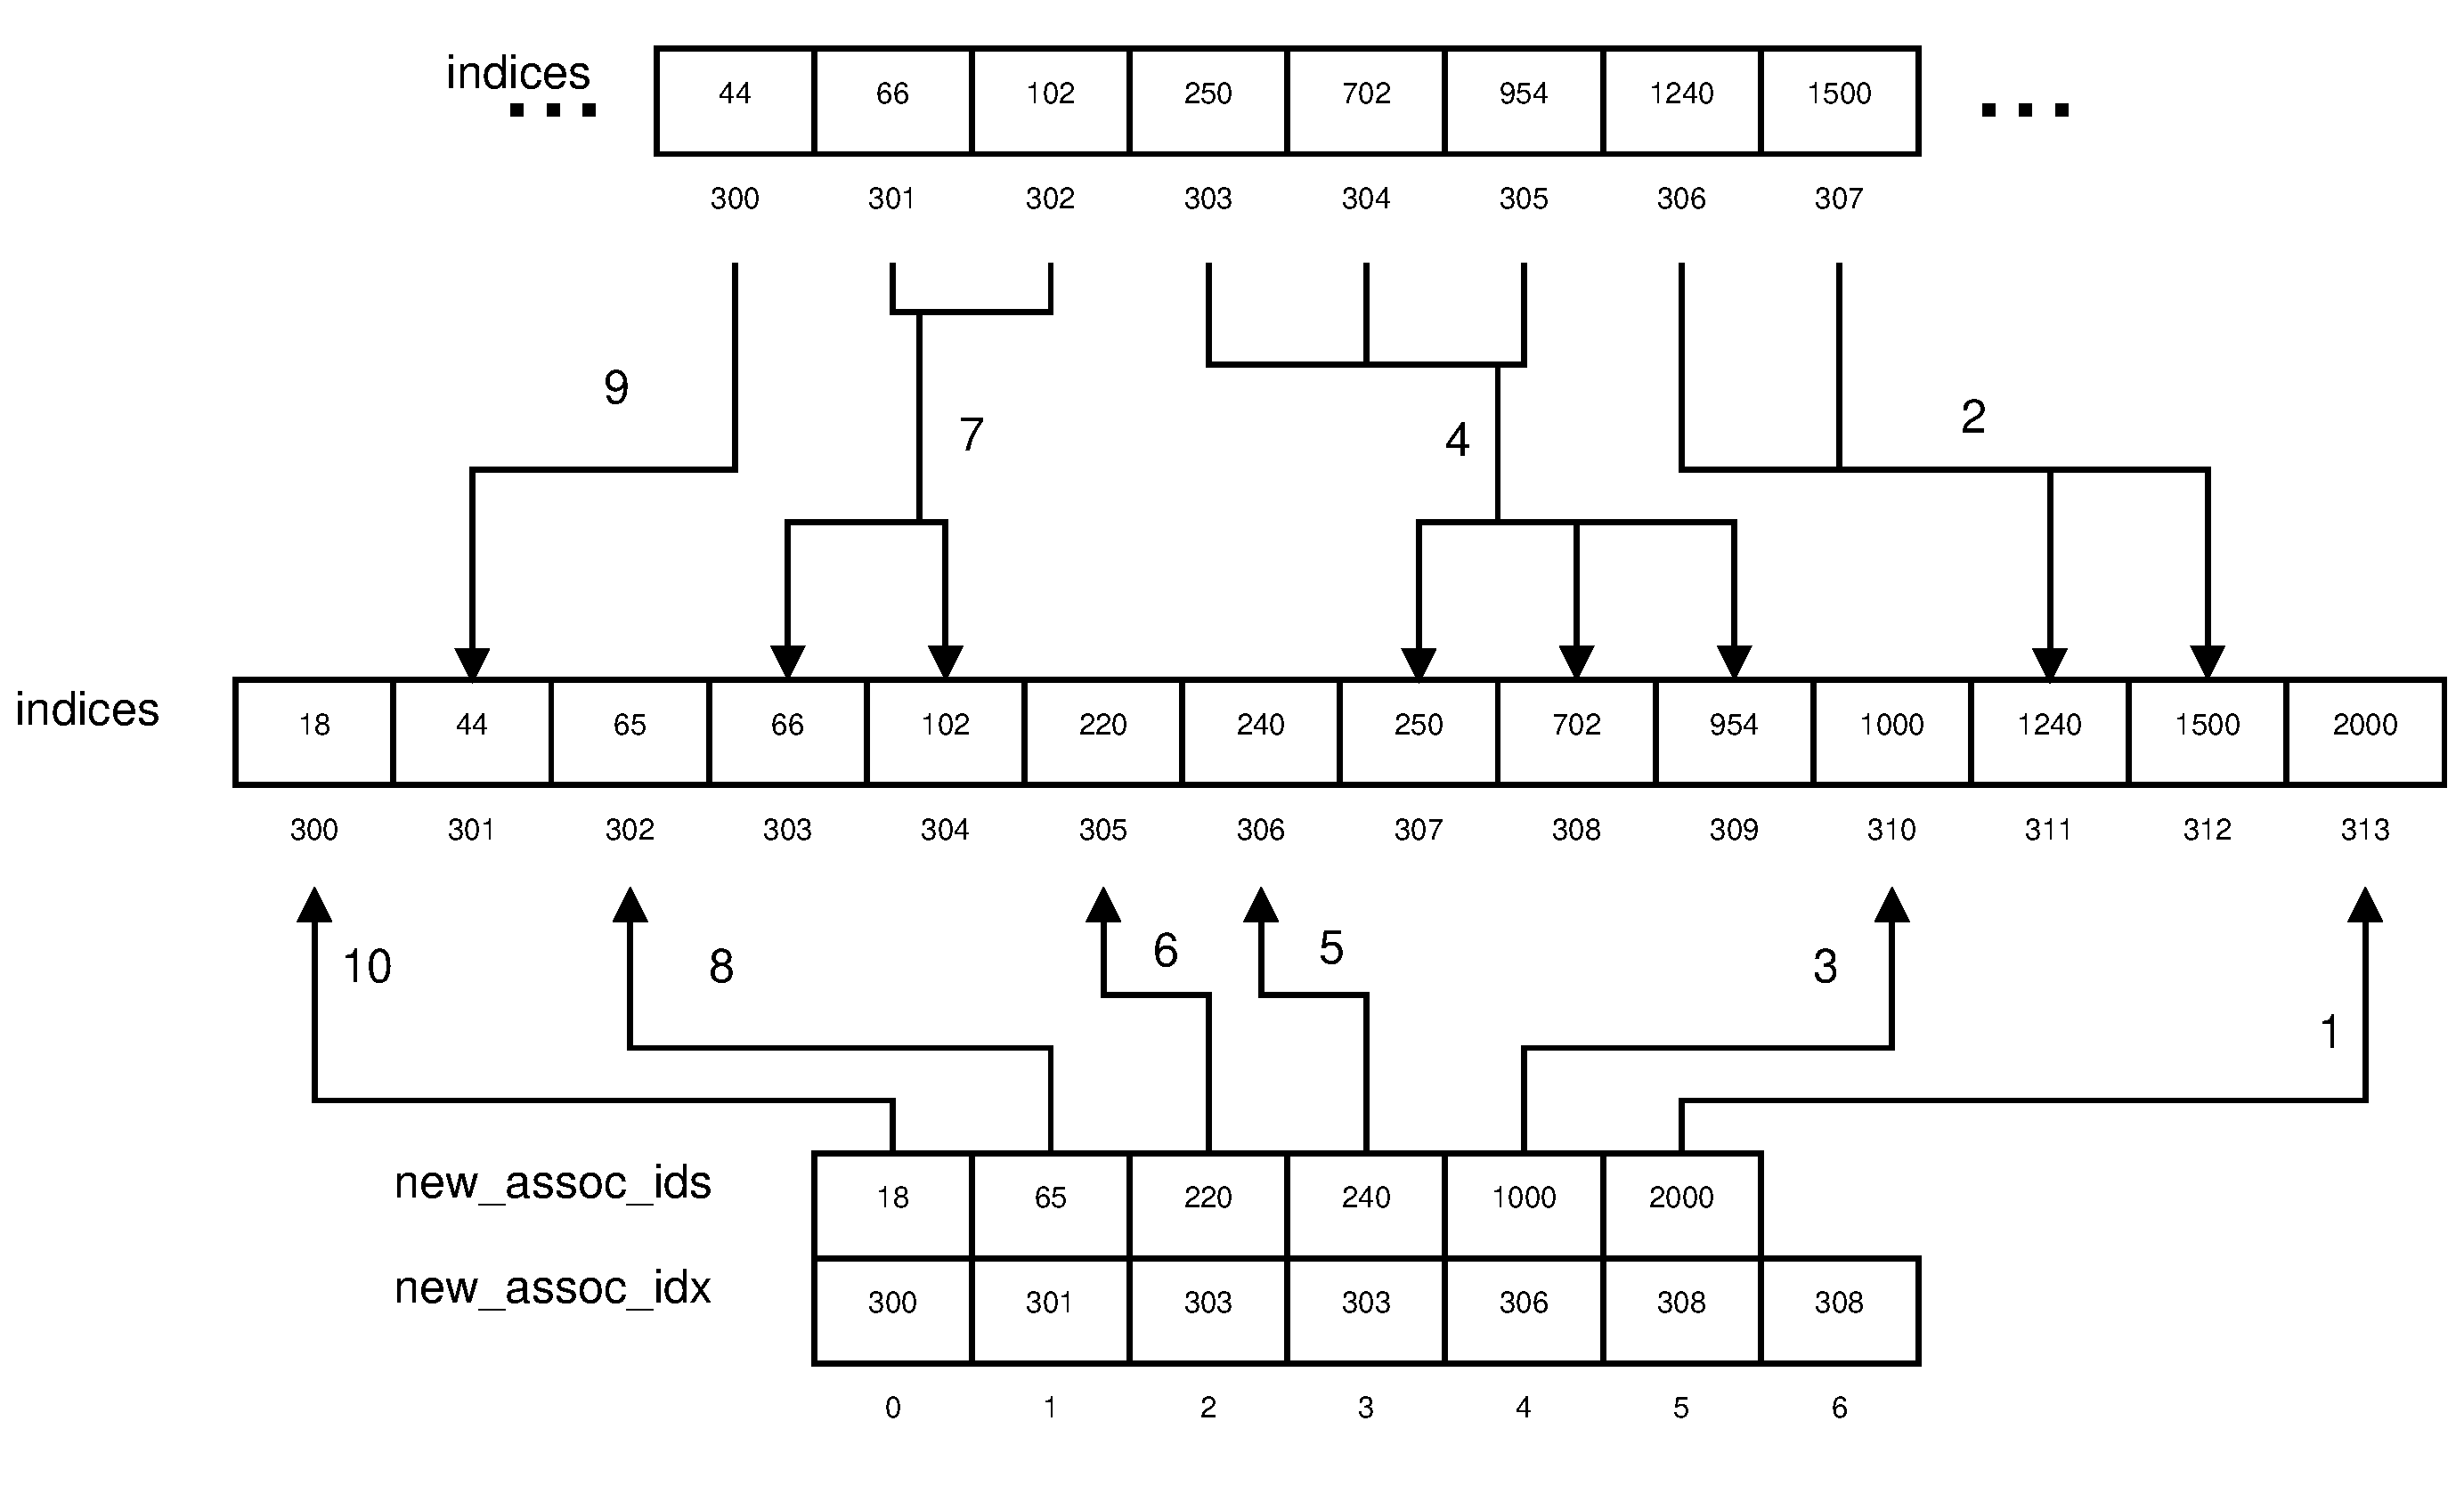
\includegraphics[width=\columnwidth]{sorted_insert}
\caption{Inserting a cluster from a partition in the co-association matrix. The arrows indicate to where the indices are moved. The numbers indicate the order of the operation.}
\label{fig:normal part}
\end{figure}


The binary search operation requires that each pattern's \emph{indices} interval be sorted.
Accordingly, new associations corresponding to each pattern are added in a sorted manner.
%New associations must be added to the pattern's  interval in a sorted manner.
%When updating a partition to the co-association matrix, the numb
%The number of associations corresponding to the $i$-th pattern (\emph{degree[i]}) is incremented by the amount of new associations to be added.
%During the sorting process a pointer to the current index to add associations $o\_ptr$ is kept (it is initialized to the new total number of associations of a pattern).
The sorting mechanism looks at the insertion indices of two consecutive new associations in the \emph{new\_assoc\_idx} array, starting from the end.
Whenever two consecutive insertion indices are not the same, it means that old associations must be moved as seen in the example.
More specifically, if the $i$-th element of the \emph{new\_assoc\_idx} array, $a$, is greater than the $(i-1)$-th element, $b$, then all the old  associations in the index interval $ \left [ a,b  \right [$ are shifted to the right by $i$ positions. %are copied to the end of the \emph{indices} interval. %, i.e. they are shifted to the right by $i$ positions.
The $i$-th element will never be smaller than the $(i-1)$-th because clusters are sorted.
Afterwards, or when two consecutive insertion indices are the same, the $(i-1)$-th element of the \emph{new\_assoc\_ids} is inserted in the position indicated by a pointer, \emph{o\_ptr}.
The \emph{o\_ptr} pointer is initiazed with the number of old associations plus the number of new asociations and is decremented anytime an association is moved or inserted.
This showed to be roughly twice as fast as using an implementation of \emph{quicksort}.


\subsection{EAC CSR Condensed}

\noindent A further reduction of space complexity in the EAC CSR scheme is possible by building only the upper triangular, since this completely describes the co-association matrix.
This means that the amount of associations decreases as one goes further down the matrix.
Instead of pre-allocating the same amount of associations for each pattern, the pre-allocation follows the same pattern of the number of associations, effectively reducing the space complexity.
The strategy used was a linear one, where the first $5\%$ of patterns have access to $100\%$ of the the estimated maximum number of associations, the last pattern has access to $5\%$ of that value and the number available for the patterns in between decreases linearly from $100\%$ to $5\%$.
\section{\uppercase{Optimization of the recovery step of EAC}}
\label{sec:recovery}

\subsection{Single-Link}

Single-Link (SL) is a Hierarchical Agglomerative Clusteirng (HAC) algorithm that has been used for the last step of EAC.
HAC algorithms operate over a pair-wise dissimilarity matrix and output a dendrogram.
The main steps of an agglomerative hierarchical clustering algorithm are \cite{Jain1999} (1) the creation of a pair-wise dissimilarity matrix of all patterns, where each pattern is a distinct cluster singleton; (2) finding the closest clusters, merge them and update the matrix to reflect this change; and, (3) repeating step 2 until all patterns belong to the same cluster.
The algorithm stops when $n-1$ merges have been performed, which is when all patterns have been connected in the same cluster.
The proximity measure between clusters in the second step distinguishes between the different HAC linkage algorithms, such as Single-Link , Average-Link, Complete-Link, among others.
In SL, the proximity between any two clusters is the the dissimilarity between their closest patterns.

An interesting property of SL, which will be relevant further on, is its equivalence with a Minimum Spanning Tree (MST) \cite{Gower1969}.
In graph theory, a MST is a tree that connects all vertices together while minimizing the sum of all the distances between them.
In the context of EAC, the edges of the MST are the distances between the patterns and the vertices are the patterns themselves.
A MST contains all the information necessary to build a SL dendrogram.
One of the advantages of using an MST based clustering is that it processes only non-zero values while a typical SL algorithm will process all pair-wise proximities, even if they are null.


%Two candidates were considered for the final step of EAC.
%A SL based on a GPU version of MST \cite{Sousa2015} was implemented.
%External algorithms were the second candidate solution.
%This solution is based on storing the co-association matrix on disk, performing the expensive computation (memory and speed wise) of \emph{argsort} and then processing the matrix in batches until the final MST is extracted.

\subsection{Kruskal's algorithm and implementation}

% Kruskal algorithm
Kruskal's algorithm was used for computing the MST.
The original paper of Kruskal's \cite{kruskal1956shortest} algorithm describes three approaches for finding a MST.
The SciPy scientific computing Python library \cite{JonesSciPy} offers an efficient implementation for the following construct (taken directly from the original paper of Kruskal's algorithm):
\begin{displayquote}
CONSTRUCTION A. Perform the following step as many times as possible: Among the edges of G not yet chosen, choose the shortest edge which does not form any loops with those edges already chosen. Clearly the set of edges eventually chosen must form a spanning tree of G, and in fact it forms a shortest spanning tree.
\end{displayquote}
If the graph $G$ if connected, the algorithm will stop before processing all edges when $|V| - 1$ edges are added to the MST, where $V$ is the set of edges.
This implementation works on a sparse matrix in the CSR format.

One of the main steps of the implementation is computing the order of the edges of the graph without sorting the edges themselves, an operation called \emph{argsort}.
To illustrate this, the \emph{argsort} operation on the array $ \left [  4 , 5 , 2 , 1, 3 \right ]$ would yield $ \left [  3 , 2 , 4, 0 , 1 \right ]$ since the the smallest element is at position 3 (starting from 0), the second smalled at position 2, etc.
This operation is much less time intensive than computing the shortest edge at each iteration.
However, the total space used is typically 8 times larger for EAC since the data type of the weights uses only one byte and the number of associations is very large, forcing the use of a 8 byte integer for the \emph{argsort} output array.
%This is the real motivation to store the co-association matrix in disk and use an external sorting algorithm.
This motivated the storage of the co-association matrix in disk and usage an external sorting algorithm.

\subsection{Kruskal's implementation with an external sorting algorithm}

The \emph{PyTables} library \cite{pytables}, which is built on top of the \emph{HDF5} format \cite{hdf5}, was used for storing the co-association matrix in graph format, performing the external sorting for the \emph{argsort} operation and loading the graph in batches for processing.
This implementation starts by storing the CSR graph to disk.
However, instead of saving the \emph{indptr} array directly, it stores an expanded version of the same length as the \emph{indices} array, where the $i$-th element contains the origin vertex (or row) of the $i$-th edge.
This way, a binary search for discovering the origin vertex becomes unnecessary.

Afterwards, the \emph{argsort} operation is performed by building a completely sorted index (CSI) \cite{AltetiAbad2007} of the \emph{data} array of the CSR matrix.
It should be noted that the arrays themselves are not sorted.
Instead, the CSI allows for a fast indexing of the arrays in a sorted manner (according to the order of the edges).
The process of building the CSI has a very low main memory usage and can be disregarded in comparison to the co-association matrix.

The SciPy implementation of Kruskal's algorithm was modified to work with batches of the graph.
This was easily implemented just by making the additional data structures used in the building of MST persistent between iterations.
The new implementation loads the graph in batches and in a sorted manner, e.g. first load a batch of the 1000 shortest edges, then a batch of the next 1000 shortest edges, etc.
Each batch must be processed sequentially since the edges must be processed in a sorted manner, which means there is no possibility for parallelism in this process.
Typically, the batch size is a very small fraction of the size of the edges, so the total memory usage for building the MST is overshadowed by the size of the co-association matrix.
The time complexity for building the CSI is higher than that of computing the \emph{argsort} operation, but the formal time complexity is not reported in the source \cite{AltetiAbad2007}.
As an example, for a $500 \: 000$ vertex graph the SL-MST approach took $54.9$ seconds while the external memory approach took $2613.5$ seconds - 2 orders of magnitude higher.
%%%%%%%%%%%%%%%%%%%%%%%%%%%%%%%%%%%%%%%%%%%%%%%%%%%%%%%%%%%%%%%%%%%%%%
% RESULTS
%%%%%%%%%%%%%%%%%%%%%%%%%%%%%%%%%%%%%%%%%%%%%%%%%%%%%%%%%%%%%%%%%%%%%%
\section{\uppercase{Results}}
\label{sec:resul}

Results presented here originated from one of three machines, that will be referred to as Alpha, Bravo and Charlie.
The main specifications of each machine are as follows:
\begin{itemize}
  \item \textbf{Alpha}: 4 GBs of main memory, a 2 core Intel i3-2310M 2.1GHz CPU and a NVIDIA GT520M with 1 GB;
  \item \textbf{Bravo}: 32 GBs of main memory, a 6 core Intel i7-4930K 3.4GHz CPU and a NVIDIA Quadro K600 with 1 GB;
  \item \textbf{Charlie}: 32 GBs of main memory, a 4 core Intel i7-4770K 3.5GHz CPU and a NVIDIA K40c with 12 GB.
\end{itemize}

%%%%%%%%%%%%%%%%%%%%%%%%%%%%%%%%%%%%%%%%%%%%%%%%%%%%%%%%%%%%%%%%%%%%%%
\subsection{GPU Parallel K-Means}

Both sequential and parallel versions of K-Means were executed over a wide spectrum of datasets varying number of patterns, features and centroids.
All tests were executed on machine Charlie and the block size was maintained constant at 512.
Whenever the number of clusters was superior to $70\%$ of the number of patterns (e.g. 800 clusters for a dataset with 1000 pattern), that particular test case was not executed.


Observing Figures \ref{fig:kmeans dim 2} and \ref{fig:kmeans dim 200}, it is clear that the number of patterns, features and clusters influence the speed-up.
For the simple case of 2 dimensions (Fig \ref{fig:kmeans dim 2}), the speed-up increases with the number of patterns.
However, there is no speed-up when the overall complexity of the datasets is low.
For 2 clusters, there is no speed-up before $100 \: 000$ patterns.
And even after that mark, the speed-up is not significant.
On the other hand, for a large number of clusters, there is speed-up for any number of patterns executed.
Not only that, that speed-up is highest for a superior number of clusters.
The reason for this is that the total amount of work increases linearly with the number of clusters but is diluted by the number of threads that can execute simultaneously.

% \begin{figure}[hbtp]
    % \centering
    % \includegraphics[width=\columnwidth]{{{2_0}}}
    % \caption{Speed-up of the labeling phase for datasets of 2 dimensions and varying the number of patterns and clusters. The dotted black line represents a speed-up of one.}
    % \label{fig:kmeans dim 2}
% \end{figure}

\begin{figure}[hbtp]
    \centering
    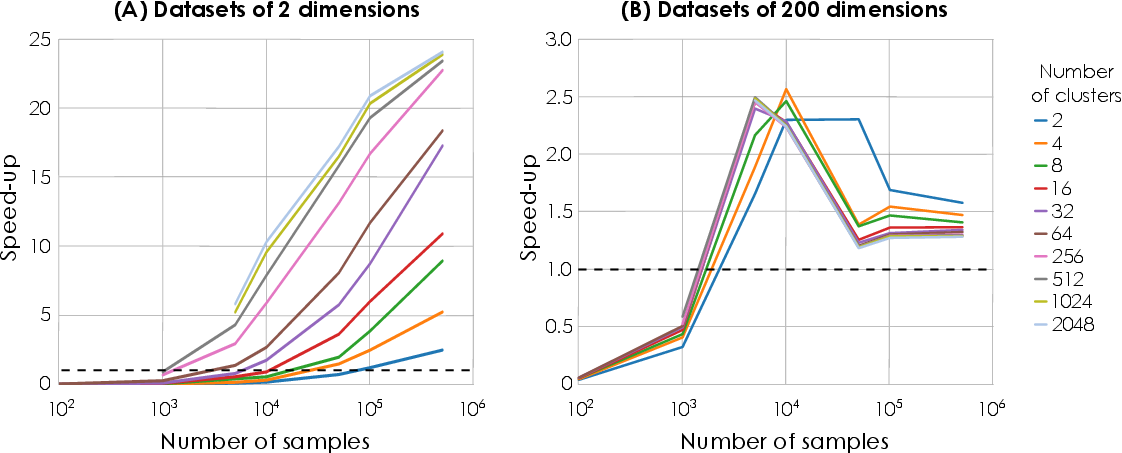
\includegraphics[width=\columnwidth]{speedup_dim}
    \caption{Speed-up of the labeling phase for datasets of 2 dimensions and varying the number of patterns and clusters. The dotted black line represents a speed-up of one.}
    \label{fig:kmeans dim 2}
\end{figure}

However, as the dimensionality increases (observe Fig. \ref{fig:kmeans dim 200}), the speed-up increases until a certain number of patterns and then decreases.
Here, the initial number of patterns for which there is a speed-up is lower and the number of clusters plays less an influence on the speed-up.
We believe the reason for this is related to the implementation itself.
The current parallel implementation does not use shared memory, which is fast.
As such, for every computation, each thread fetches the relevant data from global memory which is significantly slower.
As the number of dimensions increases, the amount of data that each thread must fetch also increases.
Furthermore, since the number of dimensions affects both data points and centroids, if the number of dimensions increases by 2 the number of fetches to memory increases by 4.
So, the speed-up increases with the dataset complexity until a point where the number of fetches to memory starts having a very significant effect on the execution time and it decreases close to $50\%$.

% \begin{figure}[hbtp]
    % \centering
    % \includegraphics[width=\columnwidth]{{{200_0}}}
    % \caption{Speed-up of the labeling phase for datasets of 200 dimensions and varying the number of patterns and clusters. The dotted black line represents a speed-up of one.}
    % \label{fig:kmeans dim 200}
% \end{figure}

%%%%%%%%%%%%%%%%%%%%%%%%%%%%%%%%%%%%%%%%%%%%%%%%%%%%%%%%%%%%%%%%%%%%%%
\subsection{Validation with original implementation}

The results of the original version of EAC, implemented in Matlab, are compared with those of the proposed solution.
Several small datasets, chosen from the datasets used in \cite{Lourenco2010} and taken from the UCI Machine Learning repository \cite{Lichman:2013}, were processed by the two versions of EAC.
Furthermore, since the generation of the ensemble is probabilistic and can change the results between runs, the proposed version is processed with the ensembles created by the original version as well.
This guarantees that the combination and recovery phases of EAC, which are deterministic when using SL, are equivalent to the original.
All data in this section refers to processing done in machine Alpha.
Table \ref{tab:validation error acc} presents the difference between the accuracies of the two versions.
Analyzing these results, it is apparent that the difference is minimal, most likely due the original version using Matlab and the proposed using Python.
Moreover, a speed-up as low as 6 and as high as 200 was obtained over the original version in the various steps, including the production step. %, even for these small datasets.

% It should be noted at this point that the original implementation always maps the dissimilarities of the co-association matrix to the range $\left [ 0 , 1 \right ]$.
% This forces the co-association matrix to have a floating point data type.
% However, since the number of partitions used is usually less than 255, the proposed version uses unsigned integers of 1 byte to reduce the used memory considerably.
% The differences in accuracy are thought to come from rounding differences of the two frameworks used and from this difference in data type.

\begin{table}[h]
\centering
\caption{Difference between accuracy of the two implementations of EAC, using the same ensemble. Accuracy was measured using the H-index \cite{Meila2003}.}

\begin{tabular}{lll}
\toprule
         &        \multicolumn{2}{c}{Number of clusters scheme} \\
Dataset &      Fixed & Lifetime \\
\midrule
breast\_cancer &  4.948755e-06 &     2.825769e-06 \\
ionosphere     &  1.652422e-06 &     1.452991e-06 \\
iris           &  3.333333e-06 &     3.333333e-06 \\
isolet         &  1.038861e-07 &     4.084904e-07 \\
optdigits      &  3.795449e-06 &     1.480513e-06 \\
pima           &  3.333333e-06 &     3.333333e-06 \\
pima\_norm     &  4.166667e-07 &     4.166667e-07 \\
wine\_norm     &  1.123596e-07 &     1.910112e-06 \\
\bottomrule
\end{tabular}

\label{tab:validation error acc}
\end{table}

%%%%%%%%%%%%%%%%%%%%%%%%%%%%%%%%%%%%%%%%%%%%%%%%%%%%%%%%%%%%%%%%%%%%%%
\subsection{Set-up for large dataset testing}
% It was suggested before that $K_{min}$ would influence other properties of EAC.
% This includes the execution times of the production, combination and recovery phases.
The results here presented refer to a synthetic large dataset comprised by a mixture of 6 Gaussians, where 2 pairs are overlapped and 1 pair is touching.
This dataset was sampled into several smaller datasets to cover a wider range of number of patterns.

Different rules for computing the $K_{min}$, different co-association matrix formats and different approaches for the final clustering will be mentioned.
The different rules and their aliases are presented in Table \ref{tab:eac rules}.
The different formats for the co-association matrix are the \emph{full} (for fully allocated $n \times n$ matrix), \emph{full condensed} (for a fully allocated $\frac{n(n-1)}{2}$ array to build the upper triangular matrix), \emph{sparse complete} (for EAC CSR), \emph{sparse condensed const} (for EAC CSR building only the upper triangular matrix) and \emph{sparse condensed linear} (for EAC CSR condensed).
The different approaches for the final clustering are \emph{SLINK} \cite{Sibson1973}, \emph{SL-MST} (for using the Kruskal implementation in SciPy) and \emph{SL-MST-Disk} for the modified version that performs an external memory sort.

\begin{table}[h]
\centering
\caption{Different rules for computing $K_{min}$ and $K_{max}$. $n$ is the number of patterns and $sk$ is the number of patterns per cluster.}

\begin{tabular}{lcc}
\toprule
Rule &  $K_{min}$ &  $K_{max}$ \\
\midrule
\emph{sqrt}     & $\frac{\sqrt{n}}{2}$      & $\sqrt{n}$    \\
\emph{2sqrt}    & $\sqrt{n}$                & $2 \sqrt{n}$  \\
\emph{sk=sqrt2} & $sk = \frac{\sqrt{n}}{2}$ & $1.3 K_{min}$ \\
\emph{sk=300}   & $sk = 300$                & $1.3 K_{min}$ \\
\bottomrule
\end{tabular}

\label{tab:eac rules}
\end{table}


The experiment that generated the results of these section was set up as follows.
A large dataset was generated.
The dataset was sampled uniformly to produce a smaller dataset with the desired number of patterns.
A clustering ensemble was produced (production phase) for each of these smaller datasets and for each of the rules, using K-Means.
From each ensemble, co-association matrices of every applicable format were built (combination phase).
A matrix format was not applicable when the dataset complexity would make its correspondent co-association matrix too big to fit in main memory.
The final clustering (recovery phase) was also done for each of the matrix formats.
The number of clusters was chosen with the lifetime criteria \cite{Fred2005}.
SL-MST was not executed if its space complexity was too big to fit in main memory.
Furthermore, the combination and recovery phases were repeated several times for smaller datasets for statistical relevant of the execution times, so as to make the influence of any background process less salient.
For big datasets, the execution times are big enough that the influence of background processes is negligible.
All results presented here originated from machine Bravo.
The same analysis that is presented here was performed on a similar dataset with separated Gaussians, from which similar conclusions were drawn.

\subsection{Execution times}

Execution times are related with the $K_{min}$ parameter, whose evolution is presented in Fig. \ref{fig:eac kmin evo}.
Rules \emph{sqrt}, \emph{2sqrt} and \emph{sk=sqrt2} never intersect but rule $sk=300$ intersects all of them, finishing with the highest $K_{min}$.
Observing Fig. \ref{fig:eac ensemble times}, one can see that the same thing happens to the production execution time associated with the $sk=300$ rule and the inverse happens to the combination time (Fig. \ref{fig:eac build rules}).
A higher $K_{min}$ means more centroids for each K-Means run to compute, so it is not surprising that the execution time for computing the ensemble increases as $K_{min}$ increases.

% \begin{figure}[hbt!]
    % \centering
    % \includegraphics[width=0.8\columnwidth]{{{kmin_evolution}}}
    % \caption{Evolution of $K_{min}$ with the number of patterns for different rules.}
    % \label{fig:eac kmin evo}
% \end{figure}

\begin{figure}[hbt!]
    \centering
    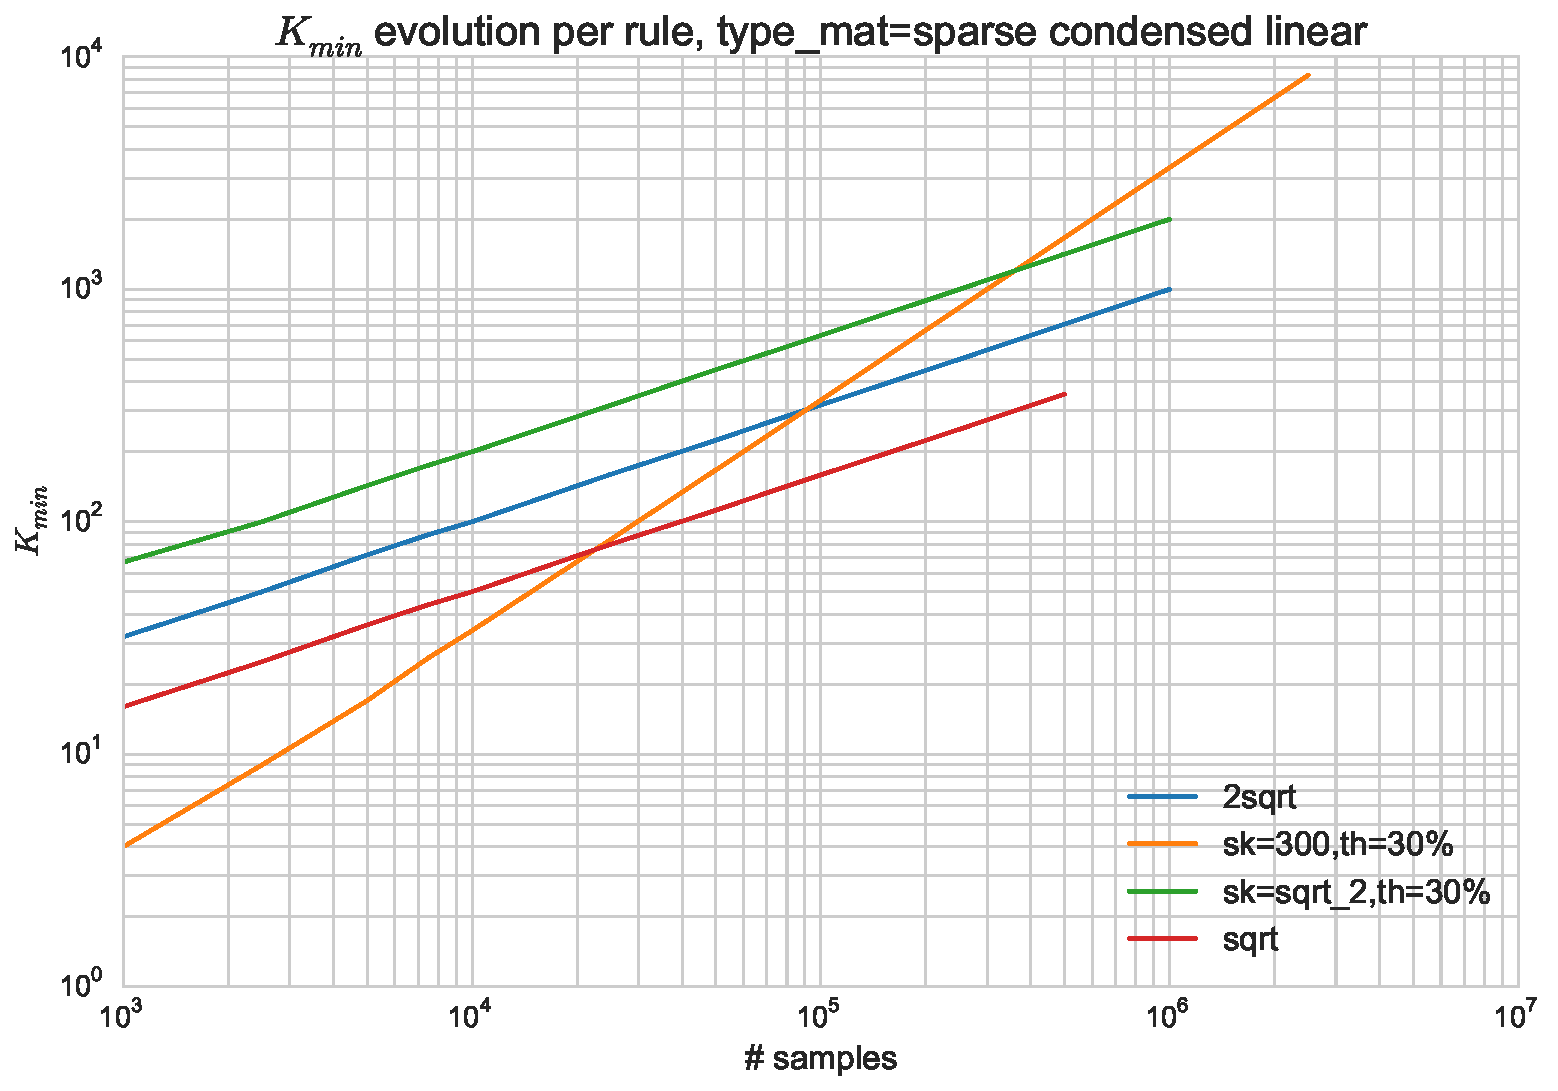
\includegraphics[width=0.55\columnwidth]{kmin_evolution}
    \caption{Evolution of $K_{min}$ with the number of patterns for different rules (type of matrix = sparse condensed linear).}
    \label{fig:eac kmin evo}
\end{figure}

\begin{figure*}[hbt!]
    \centering
    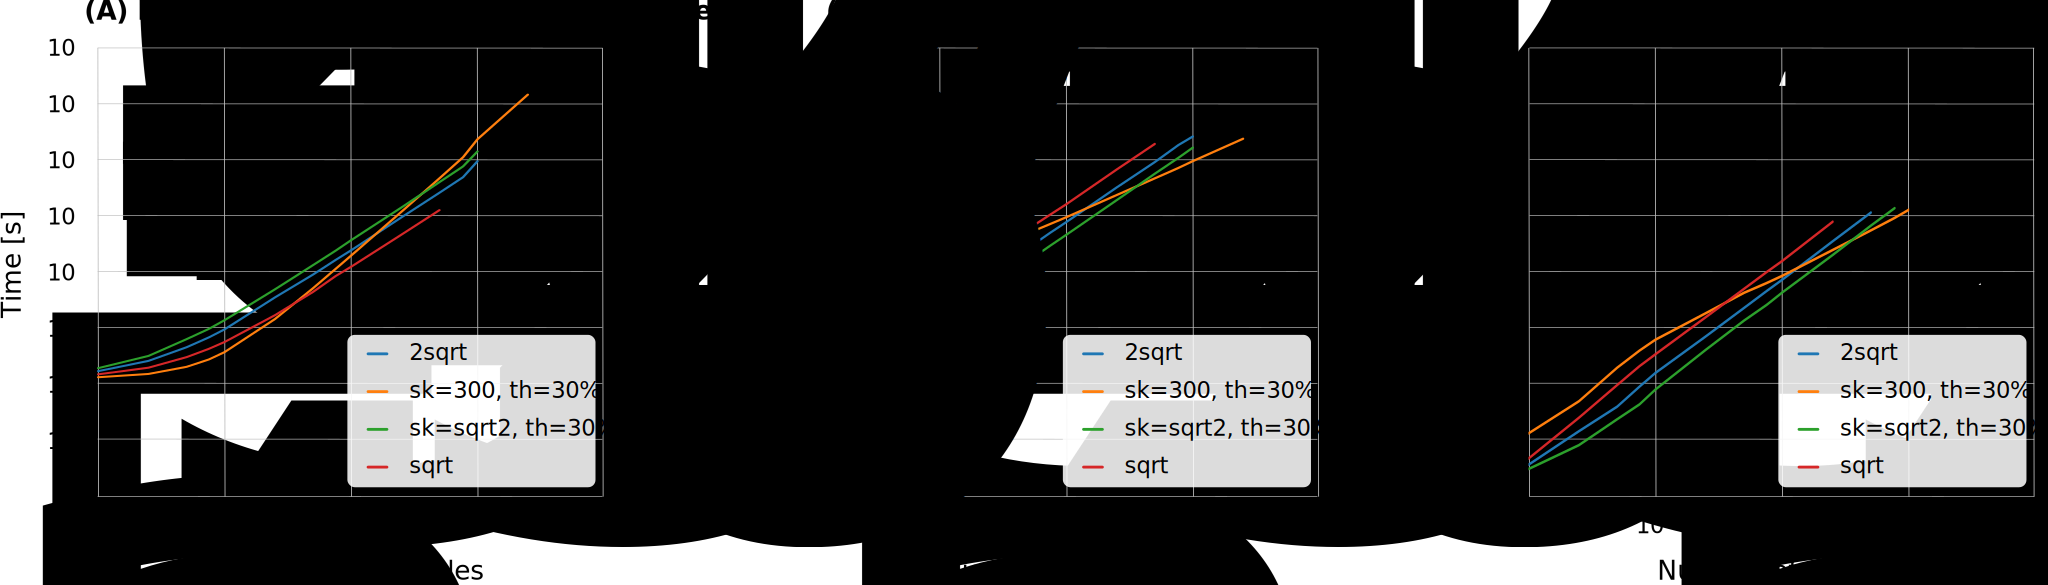
\includegraphics[width=0.8\textwidth]{execution_time_different_rules}
    \caption{Execution time with different rules for: (A) production of the clustering ensemble; (B) building the co-association matrix; and (C) extraction of the final partition with SL-MST.}
    \label{fig:eac ensemble times}
\end{figure*}

% \begin{figure}[hbt!]
    % \centering
    % \includegraphics[width=0.8\columnwidth]{{{ensemble_time}}}
    % \caption{Execution time for the production of the clustering ensemble.}
    % \label{fig:eac ensemble times}
% \end{figure}

% \begin{figure}[hbt!]
    % \centering
    % \includegraphics[width=0.8\columnwidth]{{{build_sparse_condensed_linear}}}
    % \caption{Execution time for building the co-association matrix from ensemble with different rules.}
    % \label{fig:eac build rules}
% \end{figure}

Fig. \ref{fig:eac build matrices} shows the execution times on a longitudinal study for optimized matrix formats.
It is clear that the sparse formats are significantly slower than the fully allocated ones, specially for smaller datasets.
The \emph{full condensed} format usually takes close to half the time than the \emph{full} format, which is natural given that it performs half the operations.
Idem for the \emph{sparse condensed} formats compared to the \emph{sparse complete}.
The big discrepancy between the sparse and full formats is due to the fact that the former needs to do a binary search at each association update and needs to keep the internal sparse data structure sorted.

% \begin{figure}[hbt!]
    % \centering
    % \includegraphics[width=0.8\columnwidth]{{{2sqrt}}}
    % \caption{Execution time for building the co-association matrix with different matrix formats.}
    % \label{fig:eac build matrices}
% \end{figure}

%\subsection{Performance comparison between SLINK, SL-MST and SL-MST-Disk}

The clustering times of the different methods of SL discussed previously (SLINK, SL-MST and SL-MST-Disk) are presented in Figures \ref{fig:eac sl} and \ref{fig:eac sl-mst}.
The SL-MST-Disk method is significantly slower than any of the other methods.
This is expected, since it uses the hard drive which has very slow access times compared to main memory.
SL-MST is faster than SLINK, since it processes zero associations while SL-MST takes advantage of a graph representation and only processes the non-zero associations.
In resemblance to what happened with combination times, the condensed variants take roughly half the time has their complete counterparts, since SL-MST and SL-MST-Disk over condensed co-association matrices only process half the number of associations.
Although this is not depicted, SLINK takes roughly the same time for every rule, which means $K_{min}$ has no influence.
% This comes as no surprise, since SLINK processes both zero and non-zero associations and $K_{min}$ only influences the number of non-zero associations.
This comes as no surprise, since SLINK processes the whole matrix, regardless of its association sparsity.
The same rationale can be applied to SL-MST, where different rules can have significant influence over execution time, since they change the total number of associations.
As with the combination phase, the execution time referent to the \emph{sk=300} rule started with the greatest time and decreased with an increase in the number of patterns until it was the fastest.

% \begin{figure}[hbt!]
    % \centering
    % \includegraphics[width=0.8\columnwidth]{{{slink_vs_sl-mst}}}
    % \caption{Comparison between the execution times of the three methods of SL. SLINK runs over fully allocated condensed matrix while SL-MST and SL-MST-Disk run over the condensed and complete sparse matrices.}
    % \label{fig:eac sl}
% \end{figure}

\begin{figure}[hbt!]
    \centering
    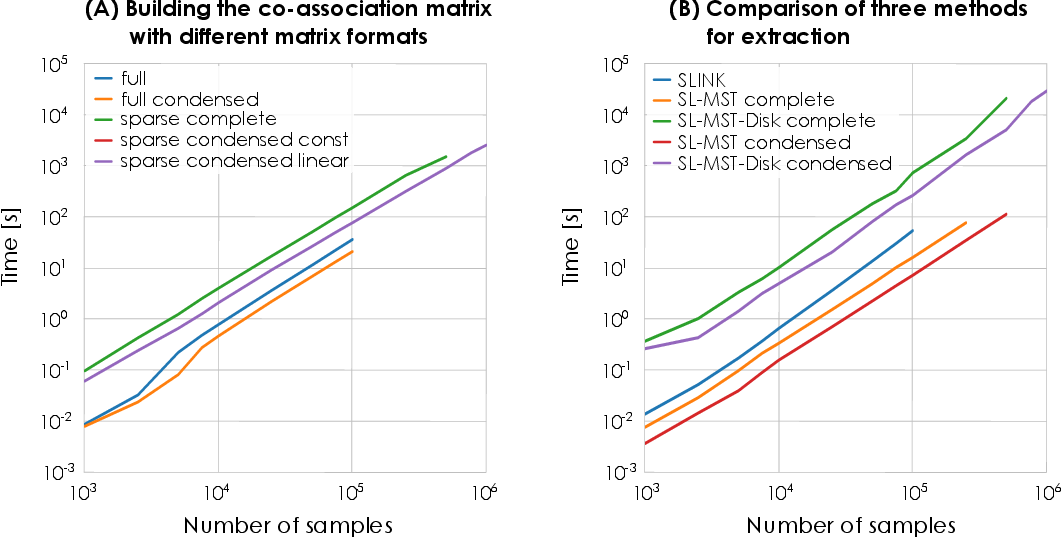
\includegraphics[width=\columnwidth]{matrix_formats_2sqrt}
    \caption{Execution time with the rule 2sqrt for: (A) building the co-association matrix with different matrix formats; and (B) comparing three methods for extraction the final partition: SLINK runs over fully allocated condensed matrix while SL-MST and SL-MST-Disk run over the condensed and complete sparse matrices.}
    \label{fig:eac sl}
\end{figure}

% \begin{figure}[hbt!]
    % \centering
    % \includegraphics[width=0.8\columnwidth]{{{sl_mem_time_sparse_condensed_linear}}}
    % \caption{Comparison between the execution times of SL-MST for different rules.}
    % \label{fig:eac sl-mst}
% \end{figure}

The execution times of all phases combined are presented in Figures \ref{fig:eac total mem} and \ref{fig:eac total disk}.
The results are presented for the \emph{sparse condensed linear} format but the remaining results follow the same pattern.
It is interesting to note that, when using the SL-MST method in the recovery phase, the execution time for three of the rules do not differ much.
This is due to a sort of balancing between a slowing down of the production phase and a speeding up of the combination and recovery phases as the $K_{min}$ increases at a higher rate for $sk=300$ than for other rules.
This is not observed for the $sqrt$ rule as $K_{min}$ is always low enough that the total time is always dominated by the combination and recovery phases.
The same does not happen when using the SL-MST-Disk method, as the total time is completely dominated by the recovery phase.
This is clear, since the results in Fig. \ref{fig:eac total disk} follow a pattern similar to that presented in Fig. \ref{fig:eac sl-mst}.

\begin{figure}[hbt!]
    \centering
    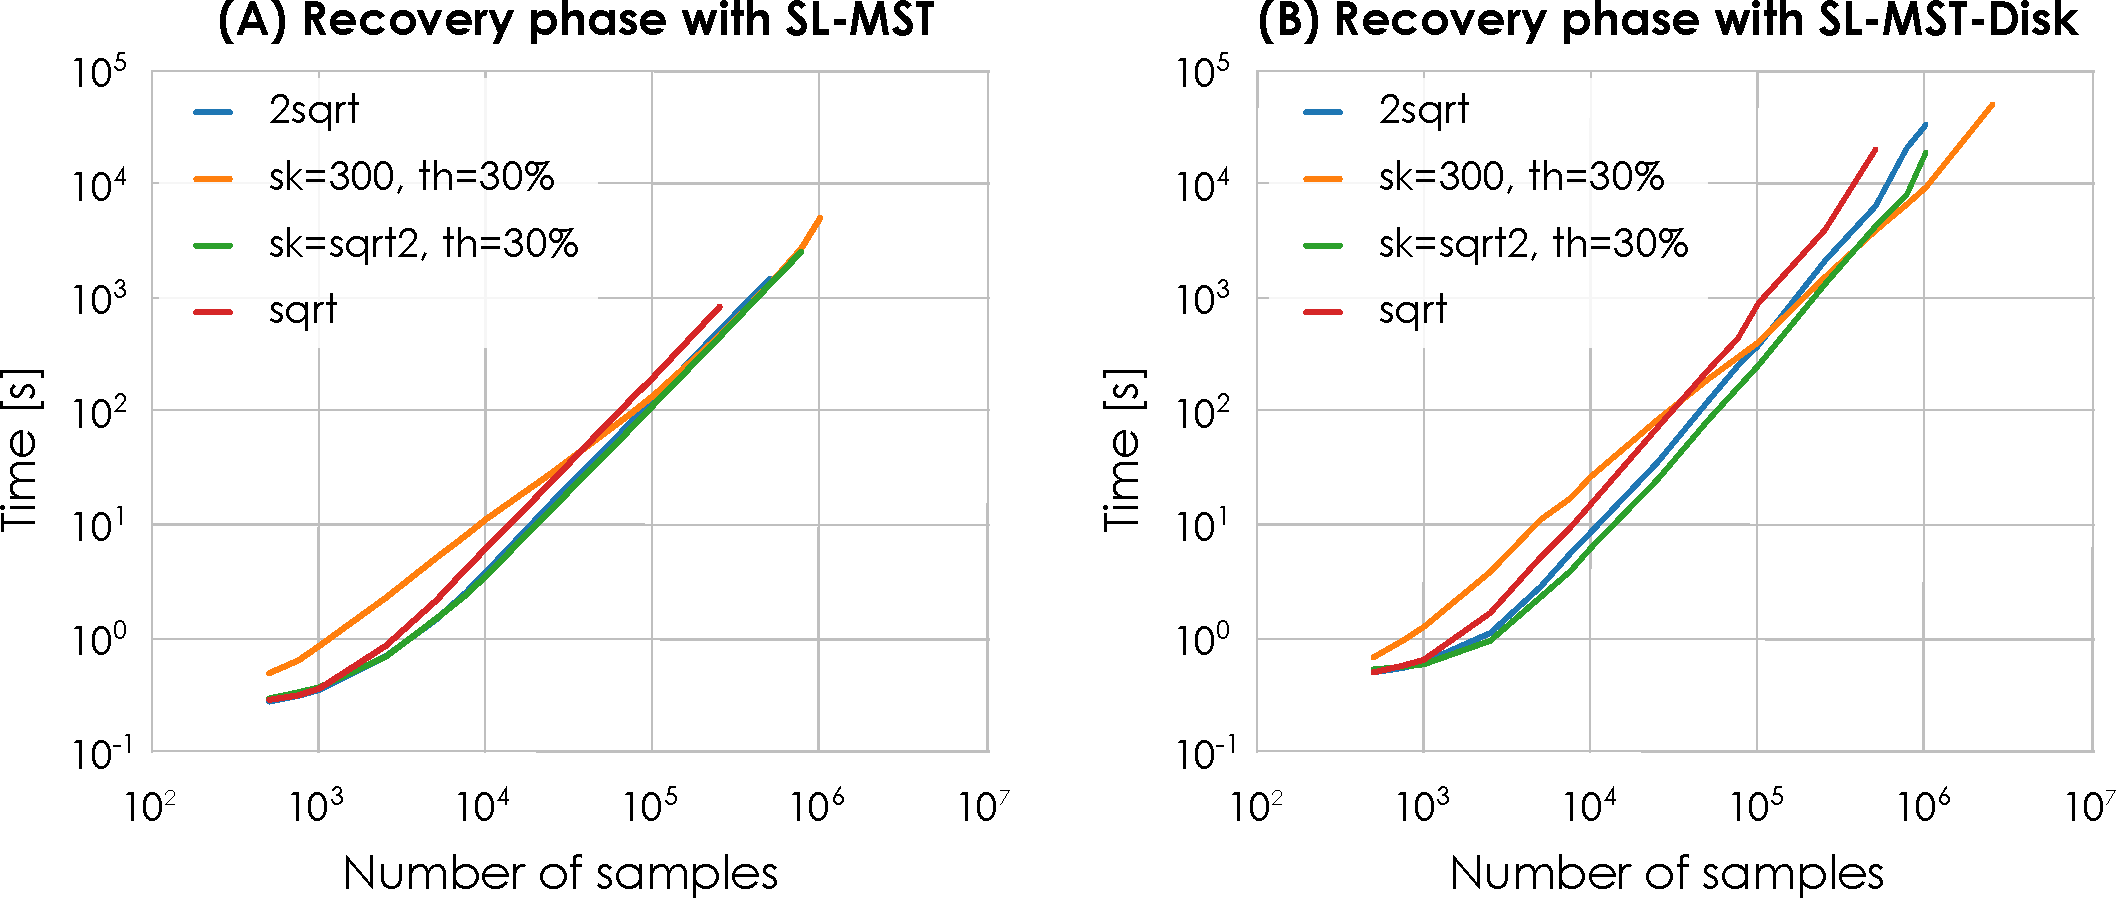
\includegraphics[width=\columnwidth]{total_execution_time}
    \caption{Execution times for all phases combined, using (A) SL-MST and (B) SL-MST-Disk in the recovery phase.}
    \label{fig:eac total mem}
\end{figure}

% \begin{figure}[hbt!]
    % \centering
    % \includegraphics[width=0.8\columnwidth]{{{total_time_sl-mst}}}
    % \caption{Execution times for all phases combined, using SL-MST in the recovery phase.}
    % \label{fig:eac total mem}
% \end{figure}

% \begin{figure}[hbt!]
    % \centering
    % \includegraphics[width=0.8\columnwidth]{{{total_time_sl-mst-disk}}}
    % \caption{Execution times for all phases combined, using SL-MST-Disk in the recovery phase.}
    % \label{fig:eac total disk}
% \end{figure}


\subsection{Analysis of the number of associations}

The sparse nature of EAC has been referred to before and is clearer in Fig. \ref{fig:eac assoc density}.
This figure shows the association density, i.e. number of associations relative to the $n^2$ associations in a full matrix.
The \emph{full condensed} format has a constant density of $49.5\%$.
Idem for the \emph{sparse complete} and \emph{sparse condensed} formats, as long as no associations are discarded.
The overall tendency is for the density to decrease as the number of patterns of the dataset increases, since the \emph{full} matrix grows quadratically.
Besides, it would be expected that the same associations would be grouped together more frequently in partitions and simply make previous connections stronger instead of creating new ones, if the relationship between the number of patterns and $K_{min}$ is constant.

% The sparse nature of EAC has been referred to before and is clearer in Fig. \ref{fig:eac assoc density}.
% This figure shows the association density, i.e. number of associations relative to the $n^2$ associations in a full matrix.
% The \emph{full condensed} format as a constant density of $49.5\%$ and the density of \emph{sparse complete} is two times that of the \emph{sparse condensed} formats.
% The overall tendency is for the density to decrease as the number of patterns of the dataset increases.
% This is to be expected since the \emph{full} matrix grows quadratically.
% Besides, it would be expected that the same associations would be grouped together more frequently in partitions and simply make previous connections stronger instead of creating new ones.
% Results presented in Fig. \ref{fig:eac assocs per pattern}, which presents the number of associations per pattern, suggest otherwise.
% The number of associations per pattern increases with the number of patterns of the dataset, with the notable exception of the \emph{sk=300} rule which increases until it reaches a certain limit and then stabilizes.
% This is explained by the fact that this rule is based on setting a maximum constant number ($300$) of patterns in any given cluster, while in the other rules this number increases with the number of patterns.
% The number of associations per pattern is not $300$ for the $sk=300$ rule because a pattern will be clustered with different neighbors in different partitions.
% Still, the number of neighbors doesn't change enough that the number of associations per pattern increases boundlessly.
% In fact, Fig. \ref{fig:eac assocs per pattern} suggests that the number of associations per pattern is around 3 times the upper bound on the number of patterns per cluster (strictly related to $K_{min}$).
% This is clearer for $sk=300$, but if one would trace the the number of patterns divided by $K_{min}$ for each rule, the contribution is close.
% \cite{Lourenco2010} reported that, on average, \"the overall contribution of the clustering ensemble (including unbalanced clusters) duplicates the co-associations produced in a single balanced clustering with Kmin clusters\".
% The spectrum of datasets evaluated regarding the number of patterns was smaller than that evaluated in the present work.
% The present results suggest a slightly higher value.
% So, the decrease in density is more related with the quadratic growth of the \emph{full} matrix in contrast with a linear growth of the number of associations.

\begin{figure}[hbt!]
    \centering
    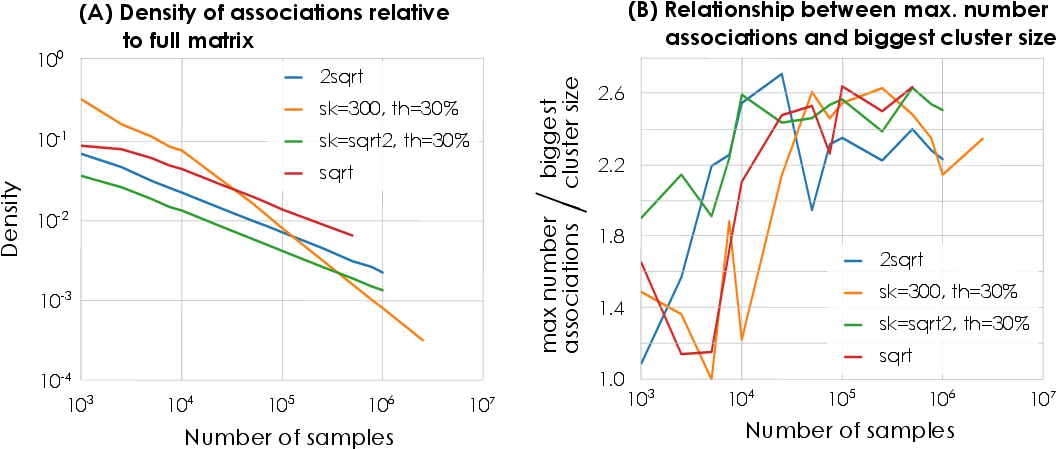
\includegraphics[width=\columnwidth]{assoc_density}
    \caption{(A) Density of associations relative to the full co-association matrix, which hold $n^2$ associations. (B) Maximum number of associations of any pattern divided by the number of patterns in the biggest cluster of the ensemble.}
    \label{fig:eac assoc density}
\end{figure}

% \begin{figure}[hbt!]
    % \centering
    % \includegraphics[width=0.8\columnwidth]{{{assoc_density_sparse_condensed_linear}}}
    % \caption{Density of associations relative to the full co-association matrix, which hold $n^2$ associations.}
    % \label{fig:eac assoc density}
% \end{figure}

% \begin{figure}[hbt!]
%     \centering
%     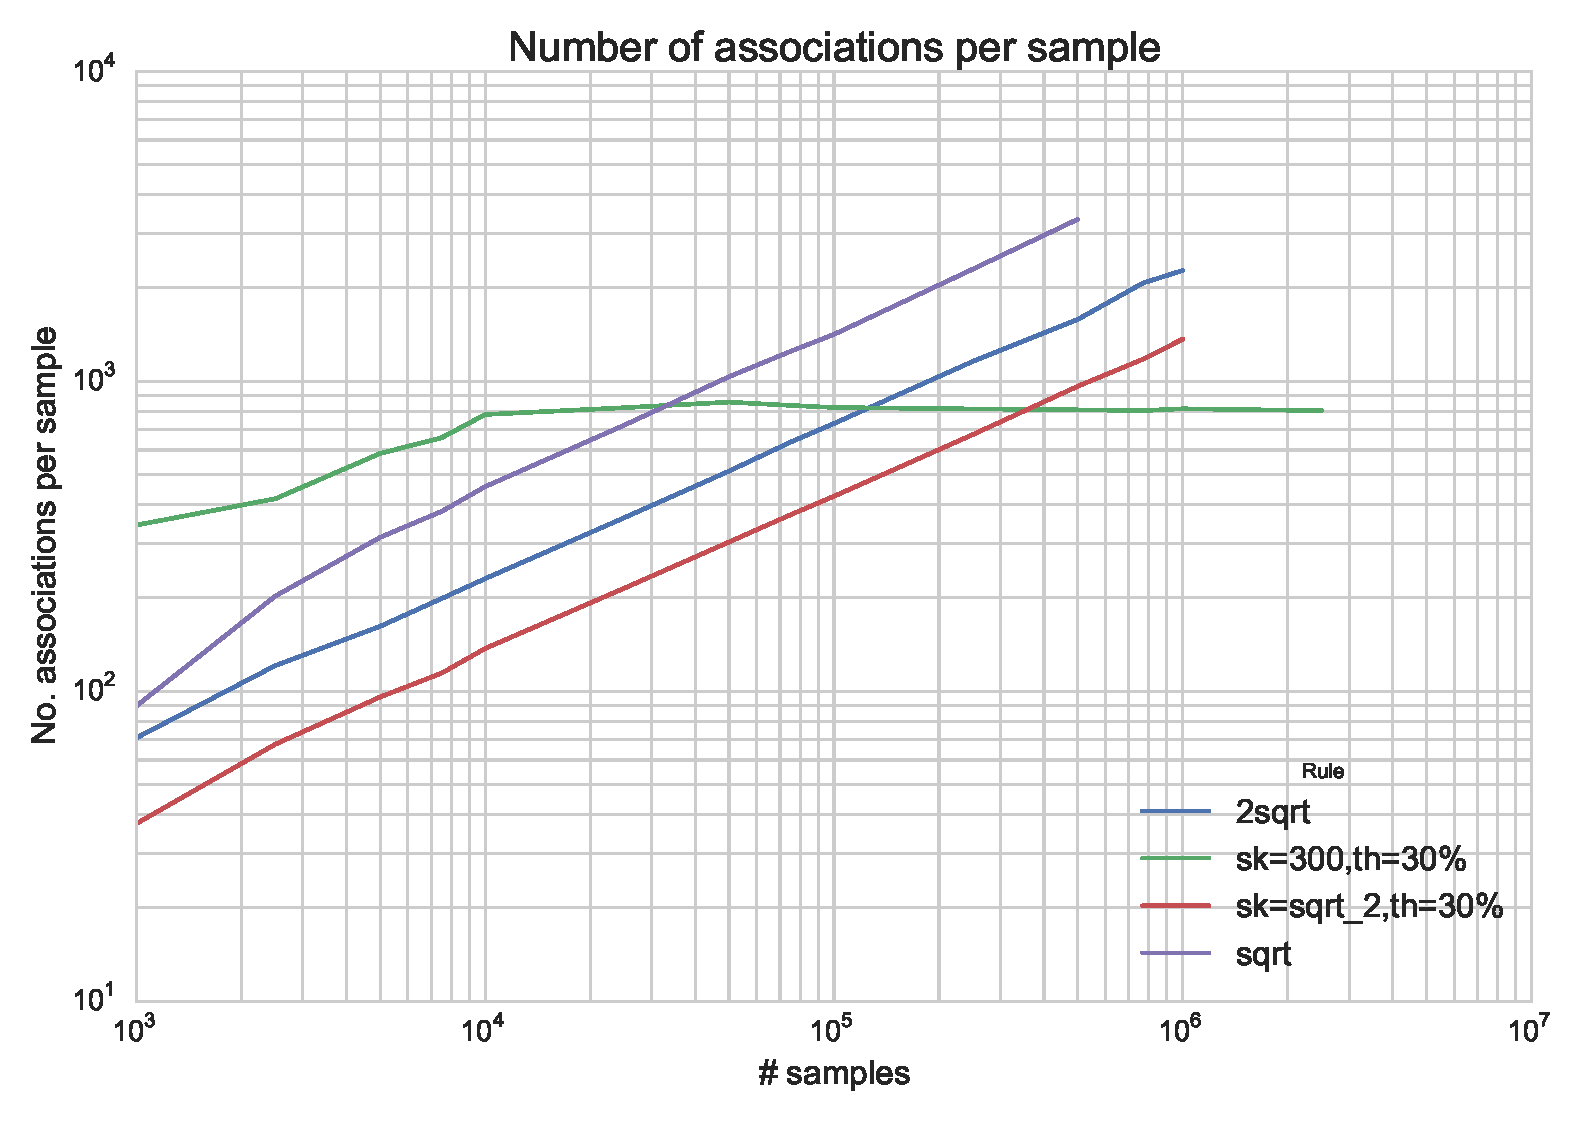
\includegraphics[width=0.8\columnwidth]{{{results/eac/assocs_per_sample}}}
%     \caption{Evolution of the total number of associations divided by the number of patterns according to the different rules.}
%     \label{fig:eac assocs per pattern}
% \end{figure}

Predicting the number of associations before building the co-association matrix is useful for coming up with combination schemes that are both memory and speed efficient.
It was stated before that the biggest cluster size in any partition of the ensemble is a good parameter for this end.
Fig. \ref{fig:eac max assocs bgs} presents the relationship between the biggest cluster size and the maximum number of associations of any pattern.
These ratio increases with the number of patterns in the beginning, but as the number of patterns increases it never goes over 3.

% \begin{figure}[hbt!]
    % \centering
    % \includegraphics[width=0.8\columnwidth]{{{max_assoc_bgs}}}
    % \caption{Maximum number of associations of any pattern divided by the number of patterns in the biggest cluster of the ensemble.}
    % \label{fig:eac max assocs bgs}
% \end{figure}

However, the number of features of the used datasets is rather reduced.
It might be the case that this ratio would increase with the number of features, since there would be more degrees where the clusters might include other neighbors.
With this in mind, further studies ranging a wider spectrum of datasets should yield more enlightening conclusions or reinforce those presented here.

\subsection{Space complexity}

As explained previously, the allocated space for the space formats is based on a prediction that uses the biggest cluster size of the ensemble.
This allocated space is usually more than what is necessary to store the total number of associations, to keep a safety margin.
Furthermore, the CSR sparse format, on which the EAC CSR strategy is based, requires an array of the same size of the predicted number of associations.
This overhead may in fact make the sparse format pre-allocate more associations than are actually possible for some rules and in very small datasets.
Still, the allocated number of associations becomes a very small fraction compared to the \emph{full} matrix as the dataset complexity increases, which is the typical case for using a sparse format.
The actual memory used is presented in Fig. \ref{fig:eac mem density}.
Here, the data types used play a big role in the amount of memory that is required.
The associations can be stored in a single byte, since the number of partitions is usually less than 255.
This means that the memory used by the fully allocated formats is $n^2$ and $\frac{n(n-1)}{2}$ Bytes for the complete and condensed versions, respectively.
In the sparse formats, the values of the associations are also stored in an array of unsigned integers of 1 Byte.
However, an array of integers of 4 bytes of the same size must also be kept to keep track of the destination pattern each association belongs to.
Besides, one other array of integers of 8 bytes is kept but it is negligible compared to the other two arrays.
The impact of the data types can be seen for smaller datasets where the total memory used is actually significantly higher than that of the \emph{full} matrix.
It should be noted that this discrepancy is not as high for other rules as for $sk=300$.
Still, the sparse formats, and in particular the condensed sparse format, is preferred since the memory used for large datasets is a small fraction of what would be necessary if using any of the fully allocated formats.

\begin{figure}[hbt!]
    \centering
    \includegraphics[width=0.8\columnwidth]{{{sk_300}}}
    \caption{Memory used relative to the full $n^2$ matrix. The \emph{sparse complete} and \emph{sparse condensed const} curves are overlapped.}
    \label{fig:eac mem density}
\end{figure}



% \section{Introduction}
% The very first letter is a 2 line initial drop letter followed
% by the rest of the first word in caps.
% 
% form to use if the first word consists of a single letter:
% \IEEEPARstart{A}{demo} file is ....
% 
% form to use if you need the single drop letter followed by
% normal text (unknown if ever used by IEEE):
% \IEEEPARstart{A}{}demo file is ....
% 
% Some journals put the first two words in caps:
% \IEEEPARstart{T}{his demo} file is ....
% 
% Here we have the typical use of a "T" for an initial drop letter
% and "HIS" in caps to complete the first word.
% \IEEEPARstart{T}{his} demo file is intended to serve as a ``starter file''
% for IEEE journal papers produced under \LaTeX\ using
% IEEEtran.cls version 1.8a and later.
% % You must have at least 2 lines in the paragraph with the drop letter
% % (should never be an issue)
% I wish you the best of success.

% \hfill mds
 
% \hfill September 17, 2014

% \subsection{Subsection Heading Here}
% Subsection text here.

% % needed in second column of first page if using \IEEEpubid
% %\IEEEpubidadjcol

% \subsubsection{Subsubsection Heading Here}
% Subsubsection text here.


% An example of a floating figure using the graphicx package.
% Note that \label must occur AFTER (or within) \caption.
% For figures, \caption should occur after the \includegraphics.
% Note that IEEEtran v1.7 and later has special internal code that
% is designed to preserve the operation of \label within \caption
% even when the captionsoff option is in effect. However, because
% of issues like this, it may be the safest practice to put all your
% \label just after \caption rather than within \caption{}.
%
% Reminder: the "draftcls" or "draftclsnofoot", not "draft", class
% option should be used if it is desired that the figures are to be
% displayed while in draft mode.
%
%\begin{figure}[!t]
%\centering
%\includegraphics[width=2.5in]{myfigure}
% where an .eps filename suffix will be assumed under latex, 
% and a .pdf suffix will be assumed for pdflatex; or what has been declared
% via \DeclareGraphicsExtensions.
%\caption{Simulation results for the network.}
%\label{fig_sim}
%\end{figure}

% Note that IEEE typically puts floats only at the top, even when this
% results in a large percentage of a column being occupied by floats.


% An example of a double column floating figure using two subfigures.
% (The subfig.sty package must be loaded for this to work.)
% The subfigure \label commands are set within each subfloat command,
% and the \label for the overall figure must come after \caption.
% \hfil is used as a separator to get equal spacing.
% Watch out that the combined width of all the subfigures on a 
% line do not exceed the text width or a line break will occur.
%
%\begin{figure*}[!t]
%\centering
%\subfloat[Case I]{\includegraphics[width=2.5in]{box}%
%\label{fig_first_case}}
%\hfil
%\subfloat[Case II]{\includegraphics[width=2.5in]{box}%
%\label{fig_second_case}}
%\caption{Simulation results for the network.}
%\label{fig_sim}
%\end{figure*}
%
% Note that often IEEE papers with subfigures do not employ subfigure
% captions (using the optional argument to \subfloat[]), but instead will
% reference/describe all of them (a), (b), etc., within the main caption.
% Be aware that for subfig.sty to generate the (a), (b), etc., subfigure
% labels, the optional argument to \subfloat must be present. If a
% subcaption is not desired, just leave its contents blank,
% e.g., \subfloat[].


% An example of a floating table. Note that, for IEEE style tables, the
% \caption command should come BEFORE the table and, given that table
% captions serve much like titles, are usually capitalized except for words
% such as a, an, and, as, at, but, by, for, in, nor, of, on, or, the, to
% and up, which are usually not capitalized unless they are the first or
% last word of the caption. Table text will default to \footnotesize as
% IEEE normally uses this smaller font for tables.
% The \label must come after \caption as always.
%
%\begin{table}[!t]
%% increase table row spacing, adjust to taste
%\renewcommand{\arraystretch}{1.3}
% if using array.sty, it might be a good idea to tweak the value of
% \extrarowheight as needed to properly center the text within the cells
%\caption{An Example of a Table}
%\label{table_example}
%\centering
%% Some packages, such as MDW tools, offer better commands for making tables
%% than the plain LaTeX2e tabular which is used here.
%\begin{tabular}{|c||c|}
%\hline
%One & Two\\
%\hline
%Three & Four\\
%\hline
%\end{tabular}
%\end{table}


% Note that the IEEE does not put floats in the very first column
% - or typically anywhere on the first page for that matter. Also,
% in-text middle ("here") positioning is typically not used, but it
% is allowed and encouraged for Computer Society conferences (but
% not Computer Society journals). Most IEEE journals/conferences use
% top floats exclusively. 
% Note that, LaTeX2e, unlike IEEE journals/conferences, places
% footnotes above bottom floats. This can be corrected via the
% \fnbelowfloat command of the stfloats package.




\section{Conclusion}
The main goal of scaling the EAC method for larger datasets than was previously possible was achieved.
In the process, it was also optimized for smaller datasets.
The EAC method is composed by three steps and, to scale the whole method, each step was optimized separately but maintaining interoperability.
In essence, the main contributions to the EAC method, by step, were the GPU parallel K-Means in the production step, the EAC CSR strategy in the combination step and the SL-MST-Disk in the recovery step.
These contributions together allow for the application of the EAC method to datasets whose complexity was not handled by the original implementation.



% if have a single appendix:
%\appendix[Proof of the Zonklar Equations]
% or
%\appendix  % for no appendix heading
% do not use \section anymore after \appendix, only \section*
% is possibly needed

% use appendices with more than one appendix
% then use \section to start each appendix
% you must declare a \section before using any
% \subsection or using \label (\appendices by itself
% starts a section numbered zero.)
%


% \appendices
% \section{Proof of the First Zonklar Equation}
% Appendix one text goes here.

% % you can choose not to have a title for an appendix
% % if you want by leaving the argument blank
% \section{}
% Appendix two text goes here.


% use section* for acknowledgment
% \section*{Acknowledgment}


% The authors would like to thank...


% Can use something like this to put references on a page
% by themselves when using endfloat and the captionsoff option.
\ifCLASSOPTIONcaptionsoff
  \newpage
\fi



% trigger a \newpage just before the given reference
% number - used to balance the columns on the last page
% adjust value as needed - may need to be readjusted if
% the document is modified later
%\IEEEtriggeratref{8}
% The "triggered" command can be changed if desired:
%\IEEEtriggercmd{\enlargethispage{-5in}}

% references section

% can use a bibliography generated by BibTeX as a .bbl file
% BibTeX documentation can be easily obtained at:
% http://www.ctan.org/tex-archive/biblio/bibtex/contrib/doc/
% The IEEEtran BibTeX style support page is at:
% http://www.michaelshell.org/tex/ieeetran/bibtex/
% \bibliographystyle{IEEEtran}
% argument is your BibTeX string definitions and bibliography database(s)
% \bibliography{IEEEabrv}
% \bibliography{library}
%
% <OR> manually copy in the resultant .bbl file
% set second argument of \begin to the number of references
% (used to reserve space for the reference number labels box)
% \begin{thebibliography}{1}

% \bibitem{IEEEhowto:kopka}
% H.~Kopka and P.~W. Daly, \emph{A Guide to \LaTeX}, 3rd~ed.\hskip 1em plus
%   0.5em minus 0.4em\relax Harlow, England: Addison-Wesley, 1999.

% \end{thebibliography}
\bibliographystyle{./bibtex/myIEEEtranS}
% \bibliography{./bibtex/IEEEabrv,./newlib4}
\bibliography{./bibtex/IEEEabrv,./library}

% biography section
% 
% If you have an EPS/PDF photo (graphicx package needed) extra braces are
% needed around the contents of the optional argument to biography to prevent
% the LaTeX parser from getting confused when it sees the complicated
% \includegraphics command within an optional argument. (You could create
% your own custom macro containing the \includegraphics command to make things
% simpler here.)
%\begin{IEEEbiography}[{\includegraphics[width=1in,height=1.25in,clip,keepaspectratio]{mshell}}]{Michael Shell}
% or if you just want to reserve a space for a photo:



% \begin{IEEEbiography}{Michael Shell}
% Biography text here.
% \end{IEEEbiography}

% if you will not have a photo at all:
% \begin{IEEEbiographynophoto}{John Doe}
% Biography text here.
% \end{IEEEbiographynophoto}

% insert where needed to balance the two columns on the last page with
% biographies
%\newpage

% \begin{IEEEbiographynophoto}{Jane Doe}
% Biography text here.
% \end{IEEEbiographynophoto}

% You can push biographies down or up by placing
% a \vfill before or after them. The appropriate
% use of \vfill depends on what kind of text is
% on the last page and whether or not the columns
% are being equalized.

%\vfill

% Can be used to pull up biographies so that the bottom of the last one
% is flush with the other column.
%\enlargethispage{-5in}



% that's all folks
\end{document}


